\documentclass[11pt]{article}
\usepackage[utf8]{inputenc}
\usepackage[T1]{fontenc}
\usepackage{microtype}
\usepackage{amsmath, amssymb}
\usepackage{graphicx}
\usepackage{booktabs}
\usepackage{enumitem}
\usepackage{float}
\usepackage[margin=1in]{geometry}
\usepackage[round]{natbib}
\usepackage[colorlinks=true, linkcolor=black, citecolor=black, urlcolor=blue]{hyperref}

\newcommand{\rstar}{30.1}
\newcommand{\thetaHz}{22.6}
\newcommand{\wbAlpha}{5.9}
\newcommand{\wbBeta}{1.24}
\newcommand{\nBase}{1000}
\newcommand{\nSweep}{500}
\newcommand{\nGrid}{15}
\newcommand{\HoneN}{171}
\newcommand{\HoneRTGeoR}{0.80}
\newcommand{\HoneRTGeoCV}{0.56}
\newcommand{\HoneRTParR}{0.83}
\newcommand{\HoneRTParCV}{0.81}
\newcommand{\HoneRTSigR}{0.57}
\newcommand{\HoneRTSigCV}{0.56}
\newcommand{\HoneRTLamSigR}{0.78}
\newcommand{\HoneRTLamSigCV}{0.75}
\newcommand{\HoneRTGeoPlusR}{0.84}
\newcommand{\HoneRTGeoPlusCV}{0.56}
\newcommand{\HoneErrGeoR}{0.81}
\newcommand{\HoneErrGeoCV}{0.80}
\newcommand{\HoneErrParR}{0.81}
\newcommand{\HoneErrParCV}{0.81}
\newcommand{\HoneErrSigR}{0.81}
\newcommand{\HoneErrSigCV}{0.81}
\newcommand{\HoneErrLamSigR}{0.81}
\newcommand{\HoneErrLamSigCV}{0.81}
\newcommand{\HoneErrGeoPlusR}{0.81}
\newcommand{\HoneErrGeoPlusCV}{0.80}
\newcommand{\PremBarrierR}{0.98}
\newcommand{\PremBarrierRho}{0.98}
\newcommand{\PremBarrierN}{9}
\newcommand{\JelevenTheta}{0.241}
\newcommand{\JelevenBoundLo}{0.231}
\newcommand{\JelevenBoundHi}{0.239}
\newcommand{\JelevenShiftSlope}{-0.05}
\newcommand{\JelevenShiftR}{0.35}
\newcommand{\bifJZeroA}{0.0247}
\newcommand{\bifJZeroB}{0.0390}
\newcommand{\bifJHiA}{0.0212}
\newcommand{\bifJHiB}{0.0283}
\newcommand{\bifJHiC}{0.0318}
\newcommand{\bifElevenA}{0.2191}
\newcommand{\bifElevenB}{0.2223}
\newcommand{\bifElevenC}{0.2765}
\newcommand{\regNormalSixty}{131}
\newcommand{\regImpSixty}{85}
\newcommand{\regNormalSeventyFive}{144}
\newcommand{\regImpSeventyFive}{70}
\newcommand{\regNormalNinety}{166}
\newcommand{\regImpNinety}{39}
\newcommand{\nTransA}{4}
\newcommand{\nTransB}{173}
\newcommand{\nTransC}{963}
\newcommand{\nTransD}{1142}
\newcommand{\landT}{20000}

\graphicspath{{./}{figures/}}
\setlength{\parskip}{3pt}
\setlength{\bibsep}{2pt}

\title{Phase-Plane Geometry Versus Structural Bifurcations: Dissociating Speed--Accuracy Control and Behavioral Failure Modes in a Reduced Cortical Decision Circuit}
\author{Ali Taghizadeh\\[2pt] Department of Mathematics and Computer Science,\\ Amirkabir University of Technology (Tehran Polytechnic), Tehran, Iran}
\date{}

\begin{document}
	\maketitle
	
	\begin{abstract}
		Biophysically grounded attractor networks link cortical microcircuit dynamics to perceptual decision-making, yet the quantitative mapping between deterministic phase-plane geometry, structural bifurcations, and stochastic behavioral failure modes remains incompletely understood. Analytical one-dimensional diffusion reductions hold only locally near pitchfork bifurcations, whereas high-dimensional spiking simulations preclude exact tracking of phase-plane separatrices and saddle eigenvalues. Here, we analyze the canonical two-population NMDA-dominated decision circuit of Wong and Wang (2006) across approximately \nTrialsTotal{} simulated trials to test how local saddle instability ($\lambda_u$), Euclidean resting-to-separatrix distance ($d$), and synaptic noise ($\sigma$) shape speed--accuracy trade-offs and dysfunctional regimes under stationary stimuli. First, by breaking parameter collinearity on a joint two-dimensional $(J_{11},J_{12})$ grid within the bistable winner-take-all regime, we show that $\lambda_u$ alone cannot predict decision speed across circuit configurations: although $\{\lambda_u,\sigma\}$ explains $R^2=\HoneRTLamSigR$ of $\log$ reaction time (RT) along a one-dimensional cross-inhibition ($J_{12}$) sweep, out-of-sample generalization across the 2D grid drops to grouped cross-validated (CV) $R^2=\ddRTLamCV$, whereas $\{J_{11},\sigma\}$ (CV $R^2=\ddRTJElCV$) and $\{J_{11},J_{12},\sigma\}$ (CV $R^2=\ddRTJJCV$) generalize accurately. This gap reflects both the strongly nonlinear mapping between $(J_{11},J_{12})$ and $(\lambda_u,d)$ (where $d$ tracks $J_{11}$ at $r=\dCorrDJeleven$) and the fact that local saddle coordinates capture only initial separatrix escape rather than post-saddle ramping to the downstream read-out bound. Second, we identify a tripartite dissociation between structural bifurcations, downstream read-out mechanics, and behavioral phenotypes: (1)~impulsive premature responses arise without resting-state destabilization across all \nRestTotal{} examined configurations and follow an empirical Kramers-like scaling with a pre-stimulus geometric barrier proxy (pseudo-$R^2=\premKPR$, grouped CV \premKPCV); (2)~indecisiveness emerges at $J_{11}\approx\JelevenBoundLo$--\JelevenBoundHi{} nA, prior to saddle-node annihilation of the choice attractors ($J_{11}=\bifElevenA$ nA), via a \emph{circuit-to-readout mismatch} wherein weakened self-excitation pulls stable choice attractors below a fixed motor threshold; and (3)~at 12.8\% coherence, standard accuracy and first-crossing RT metrics remain insensitive to the loss of winner-take-all competition at weak cross-inhibition, whereas the losing-population firing rate exposes the resulting co-activation.
	\end{abstract}
	
	\noindent\textbf{Keywords:} Perceptual decision-making; Attractor network; Phase-plane geometry; Ornstein--Uhlenbeck noise; Kramers-like escape; Excitation--inhibition balance; Bifurcation analysis.
	
	\section{Introduction}
	Perceptual decisions about noisy sensory evidence are accompanied by ramping activity in parietal and prefrontal cortical neurons consistent with the bounded accumulation of evidence to a termination threshold \citep{ShadlenNewsome2001, RoitmanShadlen2002, GoldShadlen2007, Kiani2008}. At the behavioral level, choice accuracy and reaction time (RT) distributions are classically described by drift--diffusion models \citep{RatcliffMcKoon2008, Bogacz2006, Palmer2005}. Biophysically grounded recurrent attractor networks provide a mechanistic counterpart: slow NMDA-receptor-mediated recurrent excitation \citep{Wang1999} enables competing selective neural populations to integrate sensory inputs over hundreds of milliseconds and converge toward categorical choice attractors via shared inhibition \citep{Wang2002, WongWang2006, Wong2007, WongHuk2008} (reviewed in \citealp{Deco2013}).
	
	Two complementary modeling traditions have connected these biophysical circuits to low-dimensional dynamics and cognitive dysfunction, yet each leaves an explanatory gap. First, \citet{WongWang2006} reduced the spiking network via mean-field approximations to a two-variable dynamical system governed by NMDA gating variables, whose phase-plane trajectories and transient dynamics explain time-varying evidence integration and decision confidence \citep{Wong2007, WongHuk2008, Insabato2010}. \citet{RoxinLedberg2008} further reduced two-population decision models to a one-dimensional nonlinear diffusion equation in the neighborhood of the pitchfork bifurcation where the symmetric state loses stability. While analytically insightful, this one-dimensional reduction is strictly local to the bifurcation; across wider parameter variations, trajectories evolve in a two-dimensional phase plane where non-gradient curl fluxes \citep{YeLi2021}, global separatrix geometry, and the relationship between attractor firing rates and downstream read-out bounds \citep{Kiani2008, Standage2011, Niyogi2013, Hanks2014, Standage2014} jointly influence decision formation. Second, computational psychiatry studies have linked altered cortical excitation--inhibition (E/I) balance to decision-making deficits \citep{BrunelWang2001, AbbottChance2005, Murray2014, Lam2022}. In particular, \citet{Lam2022} showed in a spiking network model that both elevated and lowered E/I ratios impair psychometric performance while producing distinct impulsive versus indecisive behavioral signatures. However, because high-dimensional spiking models do not permit direct calculation of saddle points, Jacobian eigenvalues, or stable manifolds (separatrices), it remains unclear to what extent deterministic geometric quantities of the phase plane predict stochastic decision speed and accuracy across circuit configurations, and whether behavioral regime boundaries actually coincide with structural bifurcations.
	
	Here, we address these questions in the canonical reduced two-population circuit of \citet{WongWang2006} by constructing a noise-resolved map that links deterministic phase-plane geometry to stochastic behavior across perturbations of recurrent self-excitation ($J_{11}$) and effective cross-inhibition ($J_{12}$). Because the two-variable model folds interneuron activity into effective coupling weights, $J_{11}/J_{12}$ represents an effective ratio of self-excitation to cross-inhibition rather than an explicit conductance ratio, providing a tractable two-parameter family of circuits.
	
	\paragraph{Research questions and hypotheses.} We test two specific hypotheses:
	\begin{itemize}[leftmargin=*]
		\item \textbf{H1 (Sufficiency of local saddle geometry vs.\ global circuit coordinates for decision speed).} We test whether mean RT and error rate at fixed stimulus coherence are captured by the unstable eigenvalue $\lambda_u$ of the decision saddle, the Euclidean distance $d$ from the pre-stimulus resting state to the separatrix, and noise amplitude $\sigma$. Crucially, along any one-parameter sweep (such as varying $J_{12}$ alone), geometric quantities are smooth functions of the single varied parameter, creating collinearity that prevents distinguishing genuine dynamical invariance from simple reparameterization. We therefore evaluate H1 both on a one-parameter $J_{12}$ sweep and across a joint two-dimensional $(J_{11},J_{12})$ grid within the bistable winner-take-all (WTA) regime, testing whether a single local saddle scalar ($\lambda_u$) collapses RT across distinct circuit configurations or whether global circuit coordinates governing both separatrix distance and post-saddle attractor ramping ($J_{11}$ and $J_{12}$) are required.
		\item \textbf{H2 (Alignment vs.\ dissociation between structural bifurcations and behavioral failure modes).} We test the hypothesis that boundaries between operational behavioral regimes (normal, impulsive, and indecisive) coincide with deterministic bifurcation curves shifted by noise. Examining $(J_{12},\sigma)$ and $(J_{11},\sigma)$ sweeps mechanism by mechanism, we show that this hypothesis fails in a structured manner, revealing a \emph{tripartite dissociation} between (1)~structural bifurcations and noise-driven pre-stimulus escape, (2)~saddle-node bifurcations and indecisiveness arising from a mismatch between choice-attractor scaling and a fixed downstream motor read-out threshold, and (3)~the bifurcation that eliminates WTA competition and standard first-crossing behavioral metrics under stationary asymmetric evidence.
	\end{itemize}
	
	\paragraph{Summary of contributions.} (i)~A reproducible simulation and continuation pipeline combining exact Ornstein--Uhlenbeck noise updates with deterministic phase-plane analysis. (ii)~A joint $(J_{11},J_{12})$ perturbation analysis demonstrating that the two local saddle quantities examined here ($\lambda_u$ and $d$) are insufficient to capture RT across circuits without accounting for global circuit coordinates, as RT is dominated by $J_{11}$ (which sets separatrix distance $d$ and post-saddle attractor depth) with a secondary modulation by $J_{12}$. (iii)~Demonstration that impulsive premature responses occur without resting-state destabilization and follow an empirical Kramers-like scaling with a geometric barrier proxy $d_0$. (iv)~Identification of a downstream circuit-to-readout mismatch (sub-threshold attractor trapping under a fixed motor read-out bound) as a mechanism of pre-bifurcation indecisiveness at low $J_{11}$. (v)~Demonstration that standard accuracy and first-crossing RT metrics under stationary stimuli at 12.8\% coherence remain insensitive to the loss of WTA competition at weak $J_{12}$, whereas the losing-population firing rate reveals pathological co-activation.
	
	\section{Circuit Model}
	Each selective excitatory population $i\in\{1,2\}$ is described by its slow NMDA synaptic gating variable $S_i$:
	\begin{align}
		\frac{dS_i}{dt} &= -\frac{S_i}{\tau_S}+(1-S_i)\,\gamma\,H(x_i), \qquad H(x)=\frac{ax-b}{1-\exp[-d_H(ax-b)]},\\
		x_1 &= J_{11}S_1-J_{12}S_2+I_0+J_{\rm ext}\mu_0\bigl(1+\tfrac{c'}{100}\bigr)+I_{\rm noise,1},\\
		x_2 &= J_{11}S_2-J_{12}S_1+I_0+J_{\rm ext}\mu_0\bigl(1-\tfrac{c'}{100}\bigr)+I_{\rm noise,2},
	\end{align}
	where $H(x)$ is the population current-to-rate transfer function (with gain curvature parameter denoted $d_H=0.154$~s here, corresponding to $d$ in \citealp{WongWang2006}, to avoid notation collision with the separatrix distance $d$ defined below) and $c'$ is the signed motion coherence (\%) favoring population 1. Baseline parameters follow the canonical biophysically reduced two-population parameterization of \citet{WongWang2006} (Appendix~\ref{app:params}). Synaptic background noise is modeled as an Ornstein--Uhlenbeck (OU) current filtered by fast AMPA kinetics:
	\begin{equation}
		\tau_{\rm AMPA}\,dI_{\rm noise,i}=-I_{\rm noise,i}\,dt+\sqrt{\tau_{\rm AMPA}}\,\sigma\,dW_i,\qquad \tau_{\rm AMPA}=2\ \text{ms},
	\end{equation}
	with stationary standard deviation $\sigma/\sqrt2$ and baseline amplitude $\sigma=0.02$ nA. Motion coherence levels (0, 3.2, 6.4, 12.8, 25.6, 51.2\%) match the random-dot motion discrimination task of \citet{RoitmanShadlen2002}.
	
	\section{Methods}
	\paragraph{Hybrid stochastic simulation and numerical verification.} Trials initialize at the deterministic pre-stimulus resting state (no stimulus), evolve under background noise for 500 ms of fixation, and then receive constant stimulus input for up to 2~s. Slow NMDA gating variables $S_i$ are advanced with the forward Euler scheme ($dt=0.5$ ms), while the fast OU noise currents $I_{\rm noise,i}$ are updated at each step using their \emph{exact} analytical Gaussian transition density \citep{Gillespie1996}. This hybrid integration avoids the $\approx 14\%$ stationary variance inflation produced by standard Euler--Maruyama discretization at $dt/\tau_{\rm AMPA}=0.25$. The simulation code is compiled with Numba, and trial $i$ uses the deterministic seed $s_0+i$ so that every reported value is exactly reproducible. Numerical convergence was verified across $dt\in\{1,0.5,0.25,0.1\}$ ms.
	
	\paragraph{Downstream decision criterion.} We define the smooth population firing-rate readout $r_i=S_i/(\gamma\tau_S(1-S_i))$, which equals $H(x^*)$ at any fixed point while filtering out 2~ms input fluctuations during transient dynamics. Motivated by physiological observations that LIP firing rates reach a stereotyped termination level at saccade initiation \citep{RoitmanShadlen2002, Kiani2008, Hanks2014}, a decision is registered at the first time $r_i\ge\theta$, where $\theta=0.75\,r^*=\thetaHz$ Hz is calibrated once at the baseline winning-attractor rate ($r^*=\rstar$ Hz) and held constant across parameter sweeps to model a fixed downstream motor read-out threshold \citep{Standage2011, Standage2014}. Trials are classified as \emph{correct} or \emph{error} (population 1 or 2 crosses $\theta$ first after stimulus onset), \emph{timeouts} (no crossing within 2~s), or \emph{premature} (crossing prior to stimulus onset; excluded from post-stimulus RT and accuracy). Because holding $\theta$ fixed across local circuit perturbations represents a specific hypothesis about uncompensated downstream read-out mechanics, we systematically evaluate sensitivity across threshold fractions $f\in[0.5,0.9]$.
	
	\paragraph{Deterministic phase-plane geometry and bifurcation analysis.} Fixed points are located via vectorized damped Newton--Raphson iteration from a dense multi-start grid using the analytic Jacobian and classified by their eigenvalue spectra \citep{Strogatz2015}. The separatrix (stable manifold of the decision saddle) is traced by integrating the reversed deterministic flow from the saddle along its stable eigenvector. We extract two local geometric coordinates for each bistable circuit: (1)~the unstable eigenvalue $\lambda_u>0$ at the decision saddle nearest to the resting state, and (2)~the signed Euclidean distance $d$ (in $(S_1,S_2)$ coordinates) from the pre-stimulus resting state to the stimulus-on separatrix (positive when the resting state lies in the correct basin). Bifurcation boundaries are located by bisection on changes in the number of stable fixed points and saddles, and attraction basins are mapped on a $130\times130$ grid of initial states. To analyze pre-stimulus escape from rest, we compute $d_0$, the Euclidean distance in $S$-space from the resting attractor to the nearest saddle of the stimulus-free system. Because the two-population system is non-gradient ($\nabla\times\mathbf{F}\neq 0$; \citealp{YeLi2021}), both $d$ and $d_0$ represent tractable geometric distance proxies in state space rather than conservative energy barriers or minimum-action integrals.
	
	\paragraph{Simulation experiments.}
	\emph{Baseline}: six coherences, \nBase{} trials each.
	\emph{$(J_{12},\sigma)$ sweep}: $J_{12}\in[0.015,0.085]$ nA and $\sigma\in[0.004,0.08]$ nA on a $\nGrid\times\nGrid$ grid, \nSweep{} trials per cell at 0\% and 12.8\% coherence, evaluating three read-out thresholds simultaneously.
	\emph{$(J_{11},\sigma)$ sweep}: identical $\sigma$ range over $J_{11}\in[0.215,0.285]$ nA.
	\emph{Joint $(J_{11},J_{12})$ grid}: a $\dNGrid\times\dNGrid$ grid spanning $J_{11}\in[\dJelevenLo,\dJelevenHi]$ nA and $J_{12}\in[\dJtwelveLo,\dJtwelveHi]$ nA at $c'=\dCoh\%$ across $\sigma\in\{\dSigmaList\}$ nA (\dTrials{} trials per cell and noise level). Grid bounds were selected so that every retained cell passes a deterministic check at 0\% coherence confirming the existence of a symmetric saddle on $S_1=S_2$ and two off-diagonal choice attractors whose firing rates exceed $\theta$ (the bistable WTA region). In total, approximately \nTrialsTotal{} trials were simulated.
	
	\paragraph{Operational behavioral regimes (evaluated at 12.8\% coherence).} \emph{Indecisive}: timeout rate $>20\%$. \emph{Impulsive}: (not indecisive and) accuracy $<0.65$ or premature rate $>10\%$. \emph{Other}: mean RT at 12.8\% not below RT at 0\%. \emph{Normal}: all remaining circuits. These operational cut-offs were fixed prior to mapping.
	
	\paragraph{Statistical modeling.} Reaction time is analyzed by ordinary least squares (OLS) on $\log$ mean RT ($\log\text{RT}_{\rm correct}$ on the joint 2D grid), and error/accuracy rates by binomial logistic regression on trial counts, summarized by McFadden pseudo-$R^2$. All continuous predictors are standardized. Because geometric quantities depend solely on $(J_{11},J_{12})$, observations sharing a circuit configuration at different noise levels $\sigma$ are not independent. We therefore assess generalization across the sampled grid via 5-fold \emph{grouped cross-validation} that holds out entire $(J_{11},J_{12})$ circuit configurations (all noise levels of a held-out circuit assigned to the same test fold). Note that grouped CV on a regular parameter grid evaluates interpolation across unseen circuit configurations within the tested domain rather than extrapolation beyond the grid boundaries. We report in-sample $R^2$, grouped-CV $R^2$, RMSE (in $\log$ units for RT and probability units for accuracy), and relative AIC ($\Delta$AIC within each comparison table). Premature responses pooled across the $J_{12}$ and $J_{11}$ sweeps are modeled by binomial logistic regression using the empirical Kramers-like functional form
	\begin{equation}
		\mathrm{logit}\,P_{\rm prem}=\beta_0+\beta_1\log\sigma+\beta_2\,\frac{d_0}{\sigma^{p}},
	\end{equation}
	where the exponent $p$ is profiled over a grid; this parametric family is motivated by Arrhenius--Kramers escape scaling $\exp(-\Delta U/\sigma^2)$ in gradient systems \citep{Kramers1940, Hanggi1990} while treating $d_0$ as an empirical geometric proxy. Wilson score intervals are used for binomial proportions.
	
	\section{Results}
	\subsection{Baseline phase-plane geometry and psychophysical validation}\label{sec:baseline}
	\begin{figure}[t]\centering
		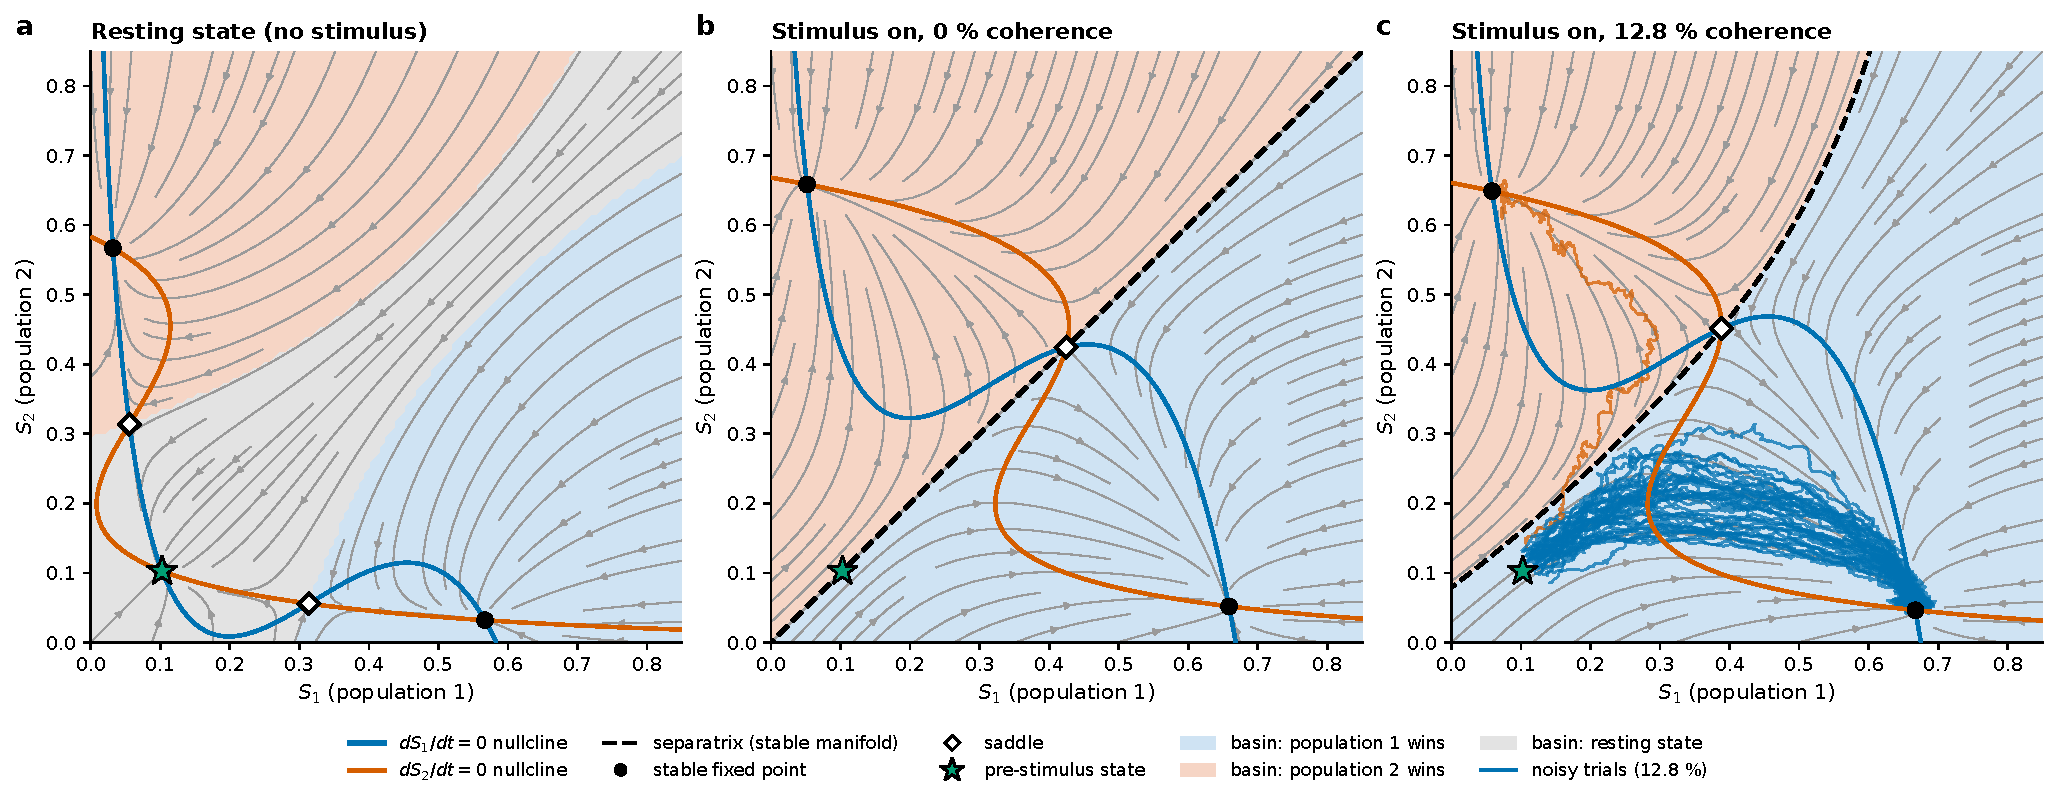
\includegraphics[width=\textwidth]{fig1_phase_portrait.pdf}
		\caption{Phase plane of the reduced model. (a) Without stimulus: stable resting state (star), two persistent memory states, and two saddles. (b) Stimulus at 0\% coherence: the resting state has vanished and the stable manifold (separatrix) of the symmetric saddle along the diagonal separates the two choice basins. (c) At 12.8\% coherence, asymmetric input shifts the saddle and separatrix; 40 stochastic trials depart the former resting state and nearly all reach the correct basin, with one error trial crossing the separatrix.}
		\label{fig:phase}
	\end{figure}
	At baseline parameters, stimulus presentation removes the low-rate resting state and leaves two stable choice attractors (winning rate \rstar{} Hz, losing rate \loserRate{} Hz) separated by a decision saddle at $S_1=S_2\approx\saddleS$ ($\approx\saddleRate$ Hz) (Fig.~\ref{fig:phase}). Individual stochastic trials ramp slowly over hundreds of milliseconds as they pass near the saddle bottleneck before diverging toward a choice attractor (Fig.~\ref{fig:behavior}a).
	
	\begin{figure}[t]\centering
		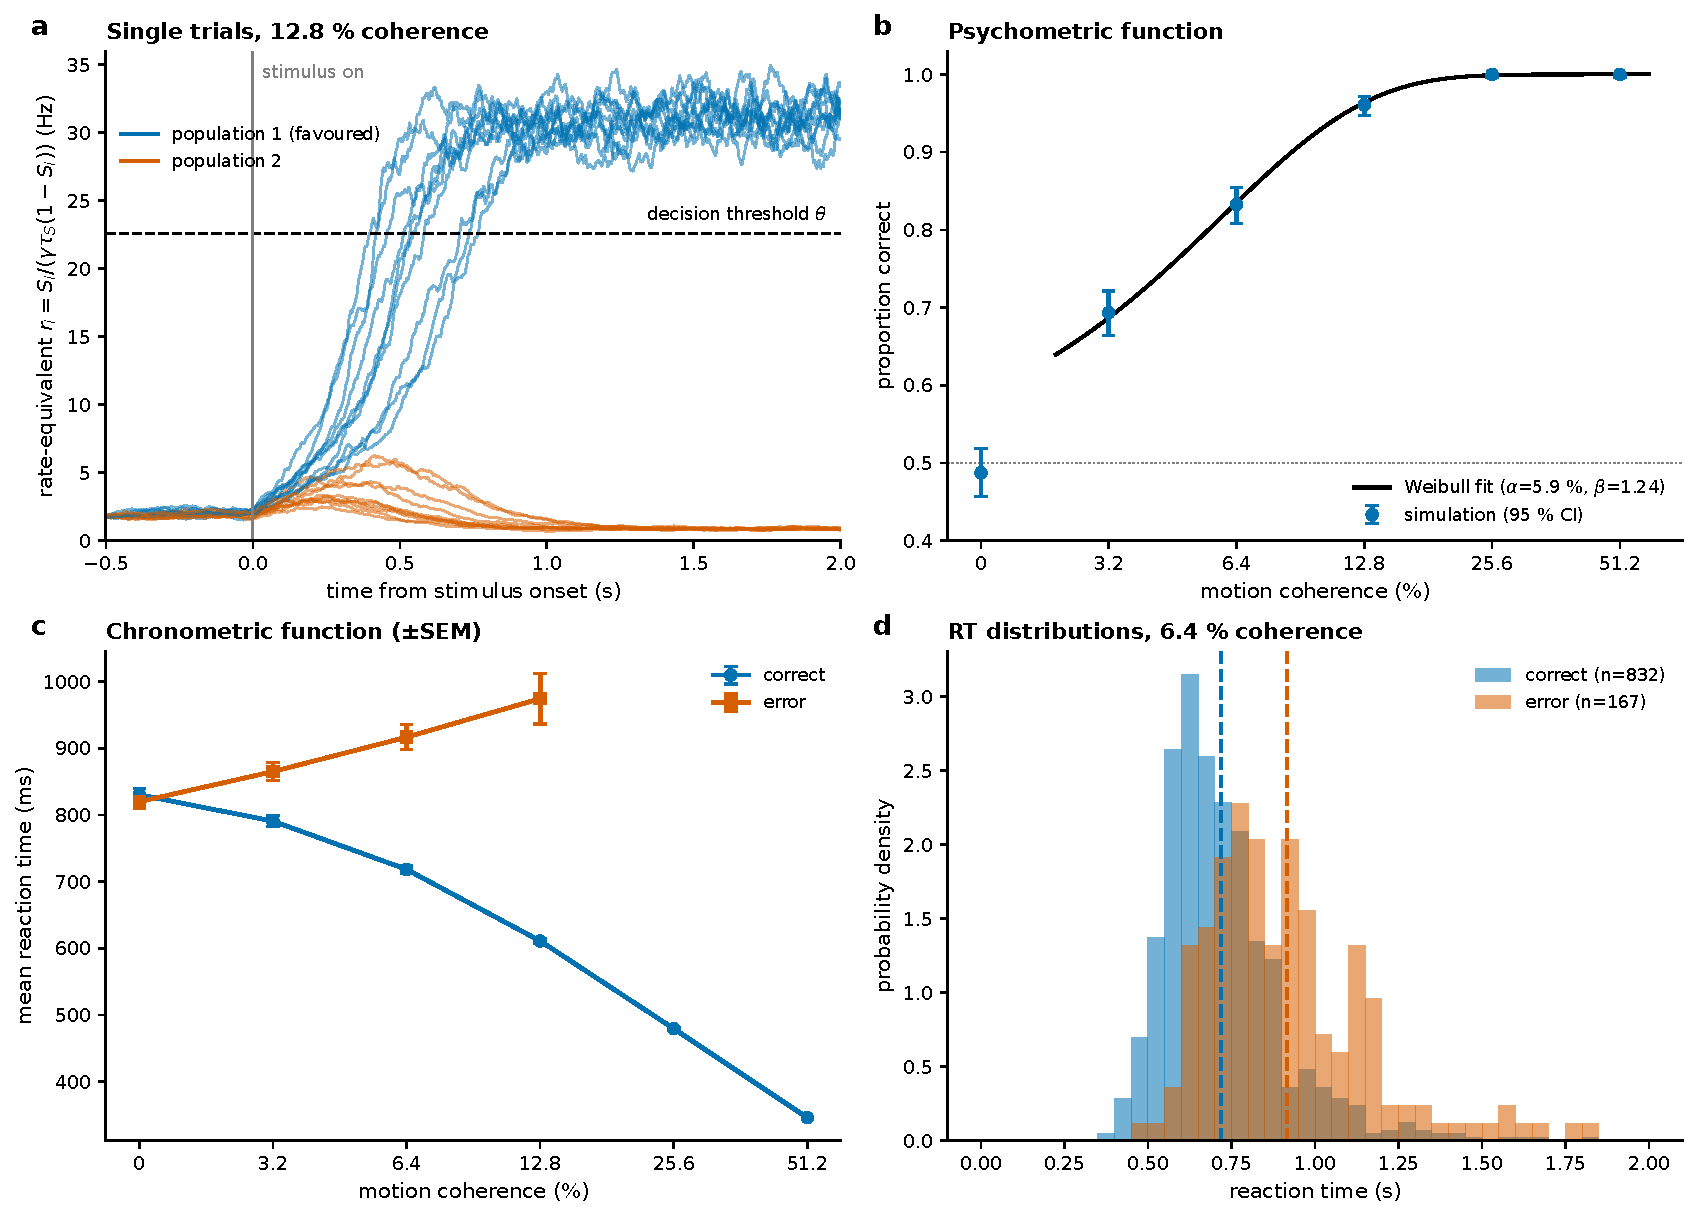
\includegraphics[width=0.92\textwidth]{fig2_behavior.pdf}
		\caption{Baseline behavior ($\sigma=0.02$ nA, \nBase{} trials per coherence). (a) Single-trial firing-rate readout traces $r_i(t)$. (b) Psychometric function with Weibull fit ($\alpha=\wbAlpha$\%, $\beta=\wbBeta$). (c) Chronometric function showing slower error responses than correct responses. (d) Right-skewed RT distributions at 6.4\% coherence.}
		\label{fig:behavior}
	\end{figure}
	\begin{table}[t]\centering\small
		\begin{tabular}{rcccc}\toprule
			Coherence (\%) & Accuracy & RT correct (ms) & RT error (ms) & Timeouts (\%)\\\midrule
			0 & 0.487 & 830 & 820 & 0.5 \\
3.2 & 0.693 & 791 & 865 & 0.5 \\
6.4 & 0.833 & 718 & 917 & 0.1 \\
12.8 & 0.961 & 611 & 974 & 0.1 \\
25.6 & 1.000 & 479 & -- & 0.0 \\
51.2 & 1.000 & 346 & -- & 0.0 \\
\bottomrule

		\end{tabular}
		\caption{Baseline summary (error RT reported only when $\ge5$ error trials occur; at 0\% coherence ``correct'' is arbitrary).}
		\label{tab:base}
	\end{table}
	Accuracy increases monotonically with motion coherence, mean RT decreases from \rtZero{} ms at 0\% to \rtMaxCoh{} ms at 51.2\%, and error trials are slower than correct trials wherever sufficient errors occur (Table~\ref{tab:base}, Fig.~\ref{fig:behavior}). These signatures match the original reduced model \citep{WongWang2006} and electrophysiological recordings in macaque area LIP \citep{RoitmanShadlen2002}. Across the four tested integration steps $dt\in\{1,0.5,0.25,0.1\}$ ms, accuracy differs by at most \dtMaxAccDiff{} and mean RT by at most \dtMaxRtDiff{} ms, within Monte Carlo sampling variability (Section~\ref{sec:sens}).
	
	\subsection{Deterministic bifurcation structure}
	\begin{figure}[t]\centering
		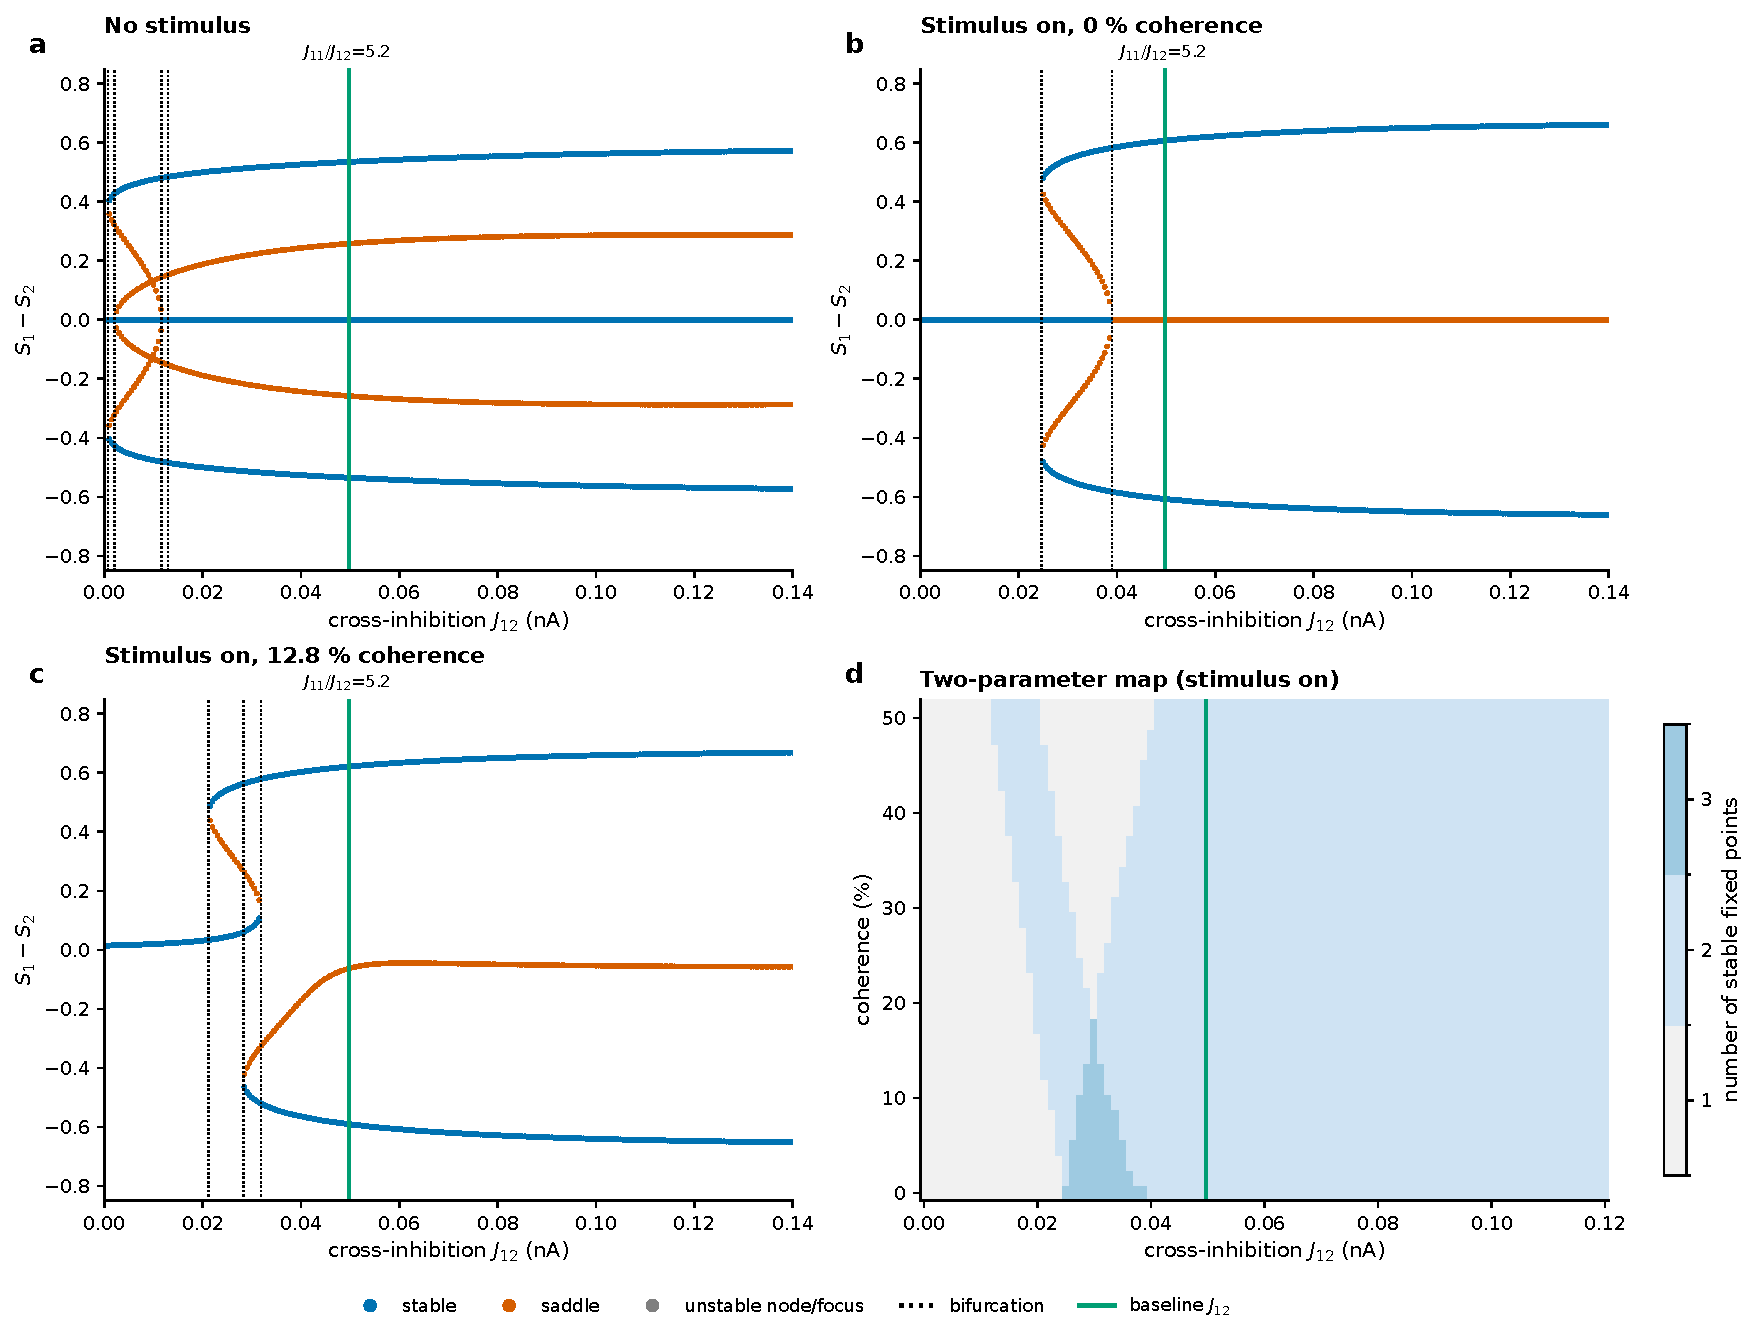
\includegraphics[width=0.95\textwidth]{fig3_bifurcation.pdf}
		\caption{Fixed-point structure versus cross-inhibition $J_{12}$ (plotted via the order parameter $S_1-S_2$). (a) Stimulus-free system. (b) Stimulus at 0\% coherence. (c) Stimulus at 12.8\% coherence, where symmetry breaking splits the bifurcation sequence. (d) Number of stable fixed points across the $(J_{12},\text{coherence})$ plane (vertical green line: baseline $J_{12}$).}
		\label{fig:bif}
	\end{figure}
	With the stimulus on at 0\% coherence, the circuit possesses a single symmetric high-rate \emph{co-activation} attractor for $J_{12}<\bifJZeroA$ nA (Fig.~\ref{fig:bif}b). At $J_{12}=\bifJZeroA$ nA, two mirror-image saddle-node bifurcations create the off-diagonal choice attractors, and at $J_{12}=\bifJZeroB$ nA the symmetric state loses stability in a subcritical pitchfork bifurcation, becoming the decision saddle of the bistable WTA regime. When stimulus symmetry is broken at 12.8\% coherence, this sequence unfolds into three distinct bifurcation events at $J_{12}=\bifJHiA$, $\bifJHiB$, and $\bifJHiC$ nA (Fig.~\ref{fig:bif}c); specifically, for $J_{12}<\bifJHiA$ nA at 12.8\% coherence, no off-diagonal choice attractors exist and only a single biased co-activation attractor remains. Along the recurrent self-excitation axis $J_{11}$ (at baseline $J_{12}$), choice attractors exist only above the saddle-node value $J_{11}=\bifElevenA$ nA (at 0\% coherence).
	
	\subsection{Operational regime map in the $(J_{12},\sigma)$ plane}
	\begin{figure}[t]\centering
		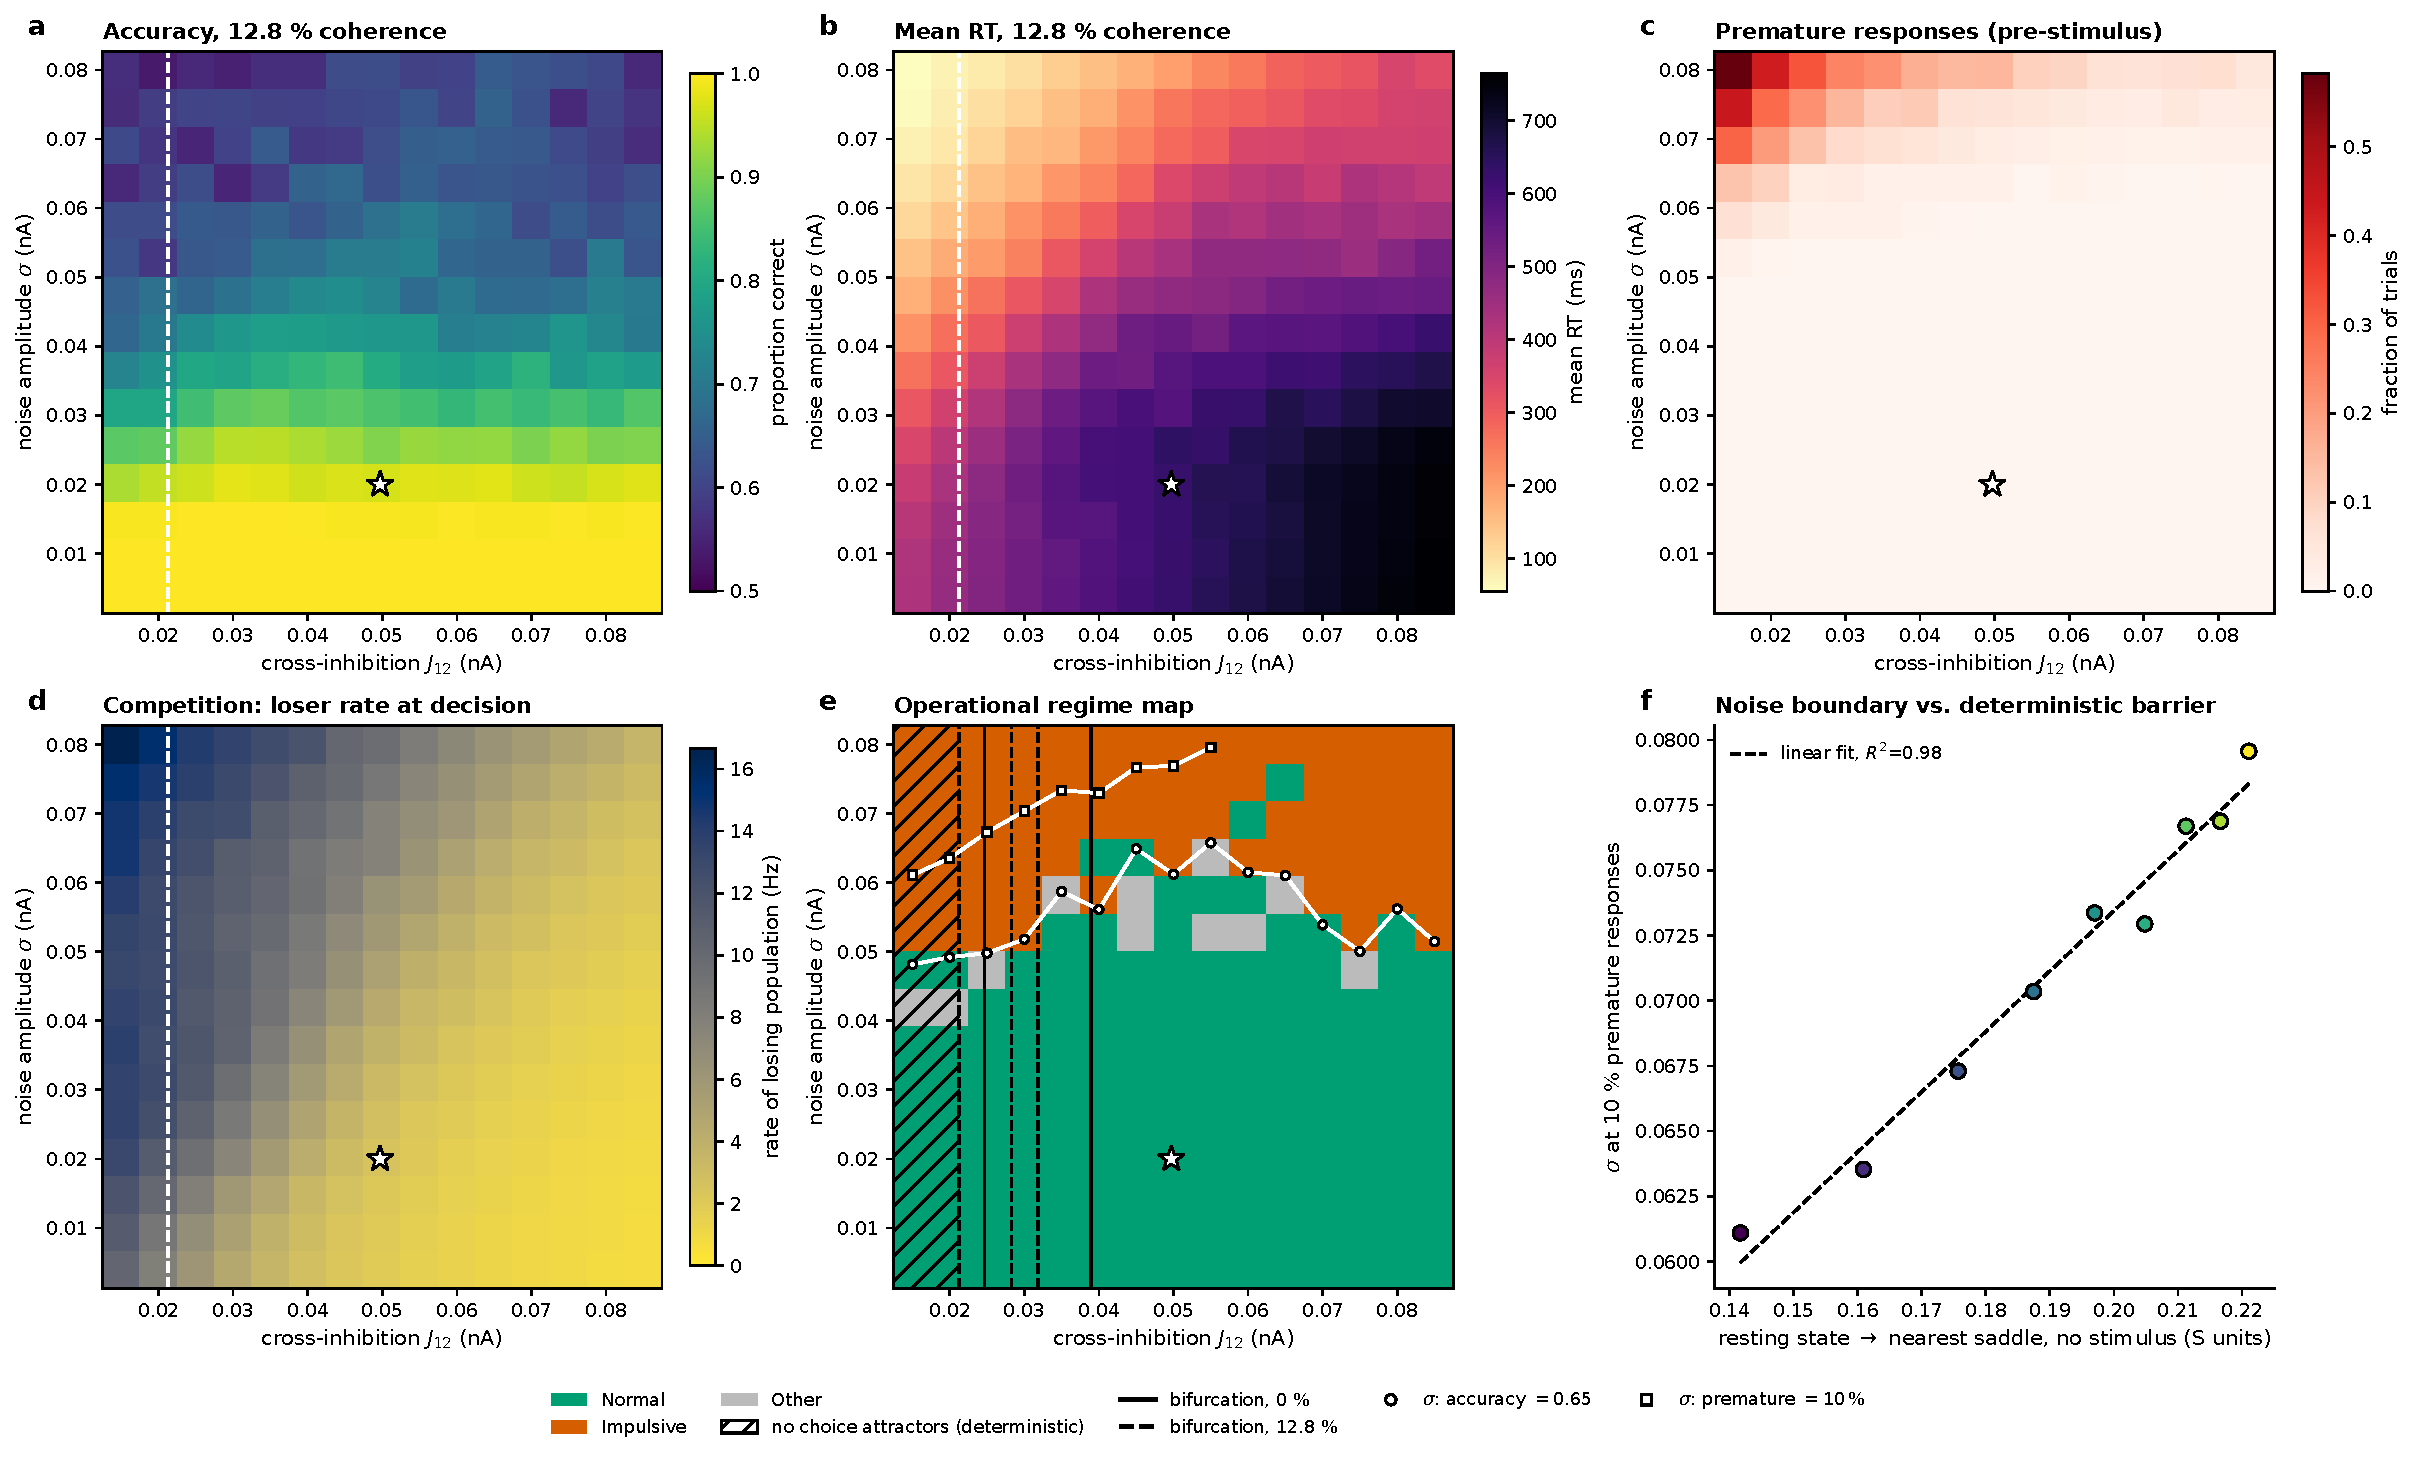
\includegraphics[width=\textwidth]{fig4_regime_map.pdf}
		\caption{Stochastic behavior over $(J_{12},\sigma)$ at 12.8\% coherence (star: baseline). (a) Choice accuracy. (b) Mean RT. (c) Premature response fraction. (d) Firing rate of the losing population at threshold crossing. (e) Operational regime map overlaid with deterministic bifurcation lines (solid: 0\% coherence; dashed: 12.8\% coherence), the hatched co-activation region lacking choice attractors at 12.8\% coherence ($J_{12}<\bifJHiA$ nA), and empirical contours where accuracy reaches 0.65 or premature responses reach 10\%. (f) Critical $\sigma$ for 10\% premature responses versus the stimulus-free geometric barrier proxy $d_0$.}
		\label{fig:regime}
	\end{figure}
	Across the $\nCells$ cells of the $(J_{12},\sigma)$ grid at 12.8\% coherence, \regNormalSeventyFive{} are classified as normal, \regImpSeventyFive{} as impulsive, \regOtherSeventyFive{} as other, and \regIndecSeventyFive{} as indecisive (Fig.~\ref{fig:regime}e). Normal task performance holds for $\sigma\lesssim 0.05$ nA across the entire $J_{12}$ range. Larger noise amplitudes degrade accuracy below 0.65, shorten RT, and drive a rising fraction of premature threshold crossings prior to stimulus onset, especially at weak $J_{12}$ (Fig.~\ref{fig:regime}c). Mean RT increases smoothly with $J_{12}$ as stronger cross-inhibition deepens the competitive bottleneck, with zero timeouts observed even at the highest $J_{12}$.
	
	\subsection{Testing H1: Geometric predictors of decision speed and accuracy}
	\subsubsection{One-parameter $J_{12}$ sweep: collinearity between saddle instability and coupling}
	\begin{figure}[t]\centering
		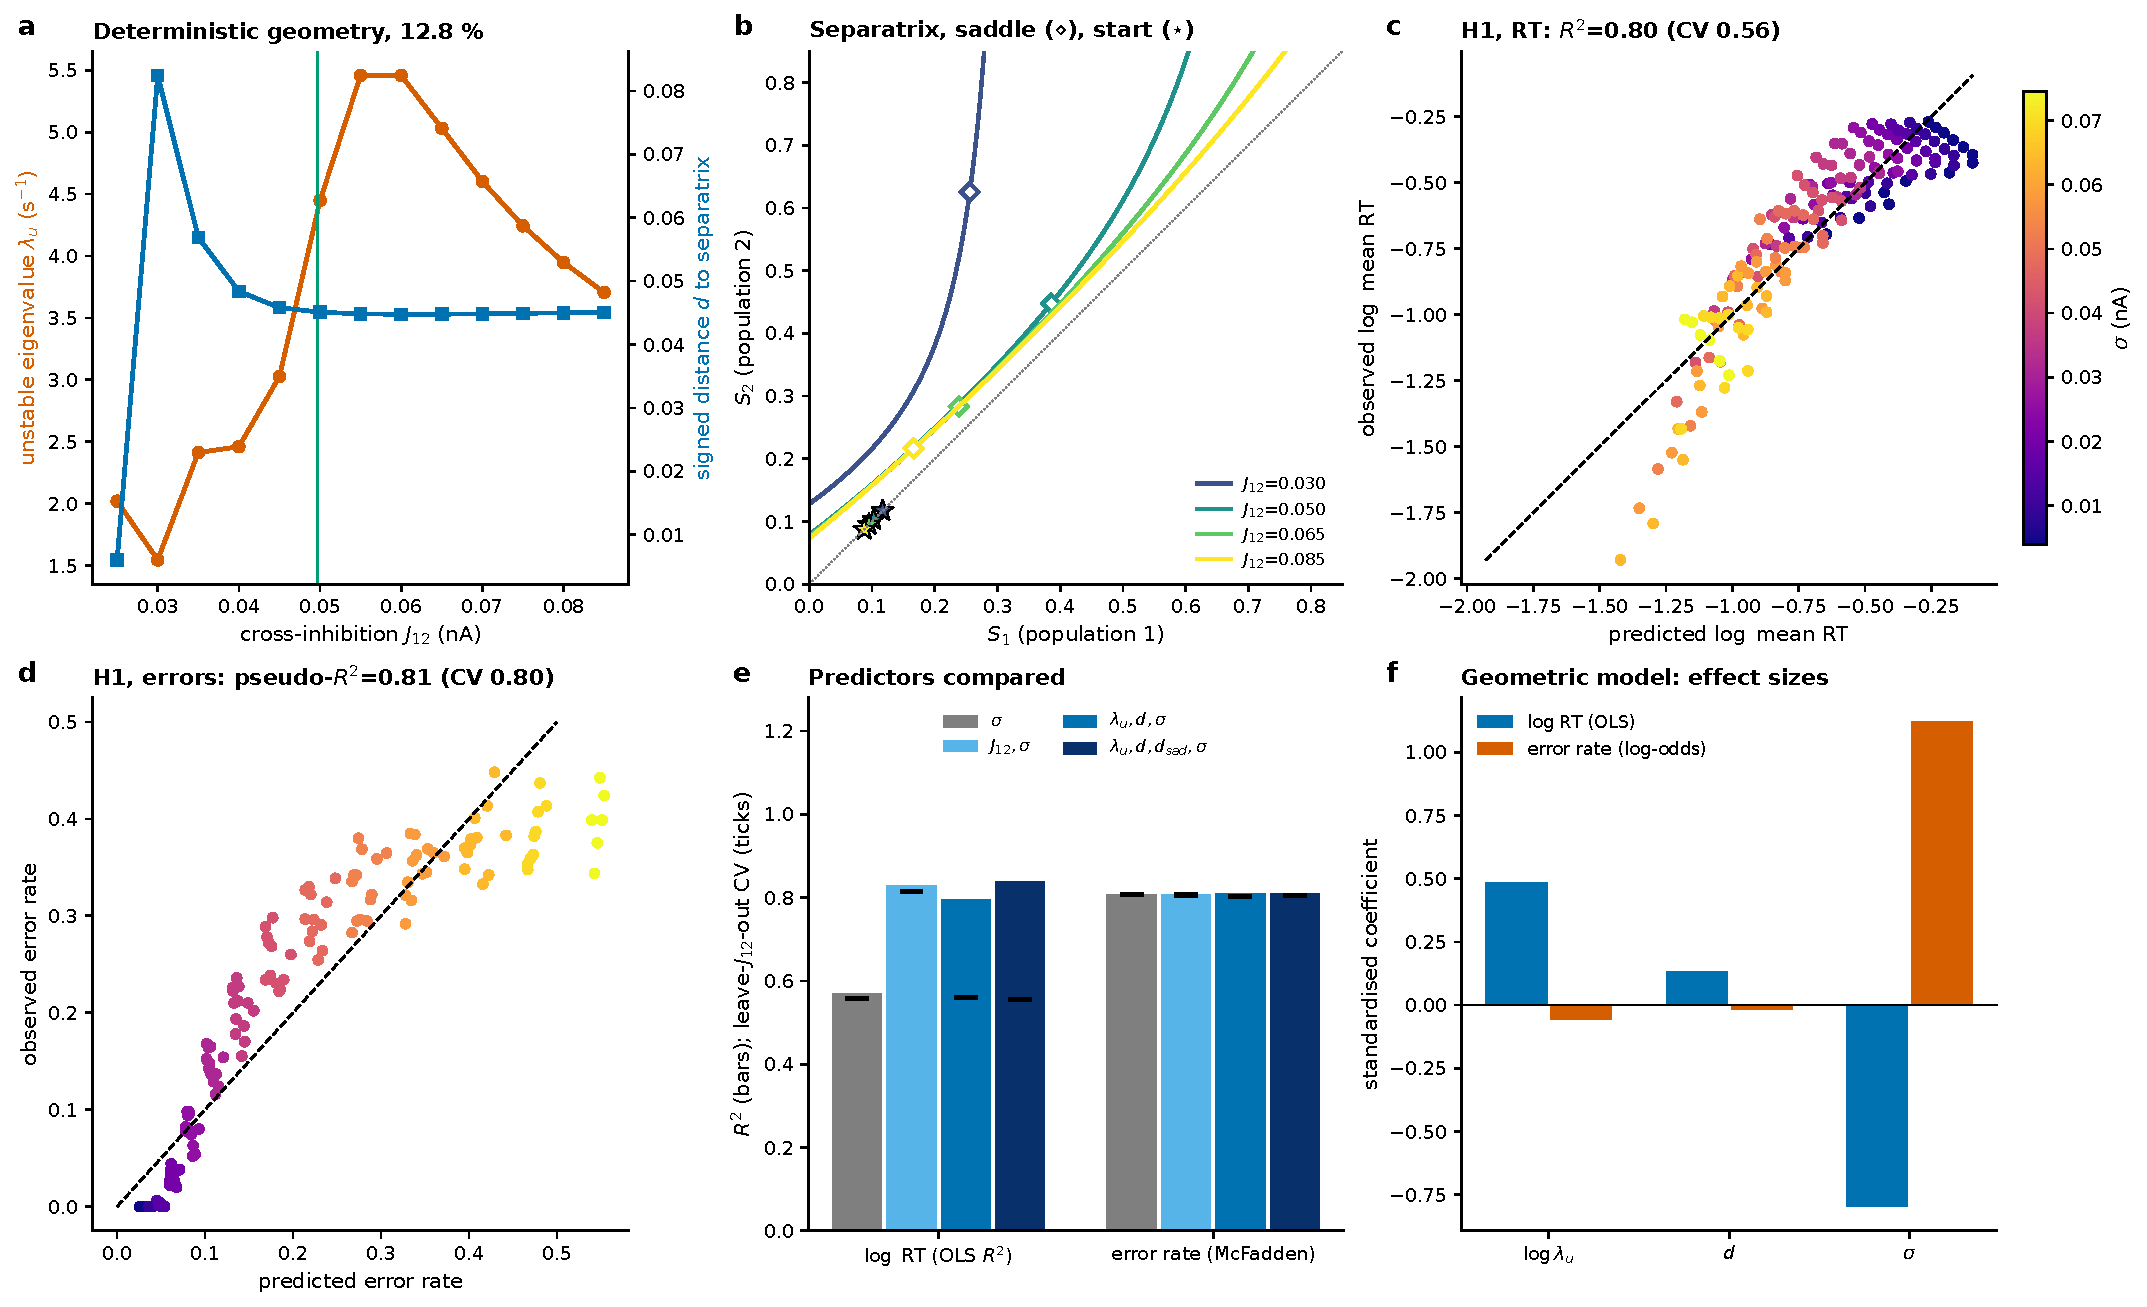
\includegraphics[width=\textwidth]{fig5_geometry_h1.pdf}
		\caption{One-parameter $J_{12}$ sweep at 12.8\% coherence. (a) Saddle unstable eigenvalue $\lambda_u$ and separatrix distance $d$ versus $J_{12}$. (b) Phase-plane separatrices, decision saddles ($\diamond$), and resting states ($\star$). (c,d) Predicted versus observed $\log$ RT and error rate for $\{\lambda_u,d,\sigma\}$. (e) In-sample $R^2$ (bars) and grouped-CV $R^2$ (ticks). (f) Standardized regression coefficients.}
		\label{fig:h1}
	\end{figure}
	\begin{table}[t]\centering\small
		\begin{tabular}{lcccc}\toprule
			& \multicolumn{2}{c}{$\log$ RT (OLS)} & \multicolumn{2}{c}{error rate (logistic)}\\
			Predictors & $R^2$ & CV $R^2$ & pseudo-$R^2$ & CV\\\midrule
			$\sigma$ & 0.57 & 0.56 & 0.81 & 0.81 \\
$J_{12},\sigma$ & 0.83 & 0.81 & 0.81 & 0.81 \\
$\log\lambda_u,\sigma$ & 0.78 & 0.75 & 0.81 & 0.81 \\
$\log\lambda_u,d,\sigma$ & 0.80 & 0.56 & 0.81 & 0.80 \\
$\log\lambda_u,d,d_{\rm sad},\sigma$ & 0.84 & 0.56 & 0.81 & 0.80 \\
\bottomrule

		\end{tabular}
		\caption{One-parameter $J_{12}$ sweep: model comparison over $n=\HoneN$ valid bistable cells; grouped CV holds out whole $J_{12}$ levels.}
		\label{tab:h1}
	\end{table}
	A decision saddle exists at 12.8\% coherence for \nGeoValid{} of the \nJtwelveGrid{} $J_{12}$ values ($n=\HoneN$ valid cells). Along this axis, $\lambda_u$ varies non-monotonically (peaking at \lamMaxVal{} s$^{-1}$ near $J_{12}=\lamMaxJ$ nA), whereas $d$ is nearly constant ($\approx\dPlateau$) for $J_{12}\ge0.045$ nA (Fig.~\ref{fig:h1}a). For $\log$ RT, noise $\sigma$ alone yields $R^2=\HoneRTSigR$; adding $\log\lambda_u$ raises this to $R^2=\HoneRTLamSigR$ (grouped CV \HoneRTLamSigCV), and removing $\lambda_u$ from the full geometric model $\{\lambda_u,d,\sigma\}$ reduces $R^2$ by $\HoneDropLam$ (Table~\ref{tab:h1}; adding $d$ adds $\HoneGainD$ in-sample but lowers grouped-CV $R^2$ to \HoneRTGeoCV{} due to high-leverage cells near the saddle-node). However, the raw parameter model $\{J_{12},\sigma\}$ performs equally well ($R^2=\HoneRTParR$, CV \HoneRTParCV). Thus, along a one-parameter sweep, $\lambda_u$ provides dynamical interpretation but cannot be statistically separated from a reparameterization of $J_{12}$. For error rate, $\sigma$ alone accounts for pseudo-$R^2=\HoneErrSigR$ and geometric predictors add less than $\HoneErrGain$.
	
	\subsubsection{Joint $(J_{11},J_{12})$ grid: local saddle instability $\lambda_u$ alone fails to collapse RT}
	\begin{figure}[t]\centering
		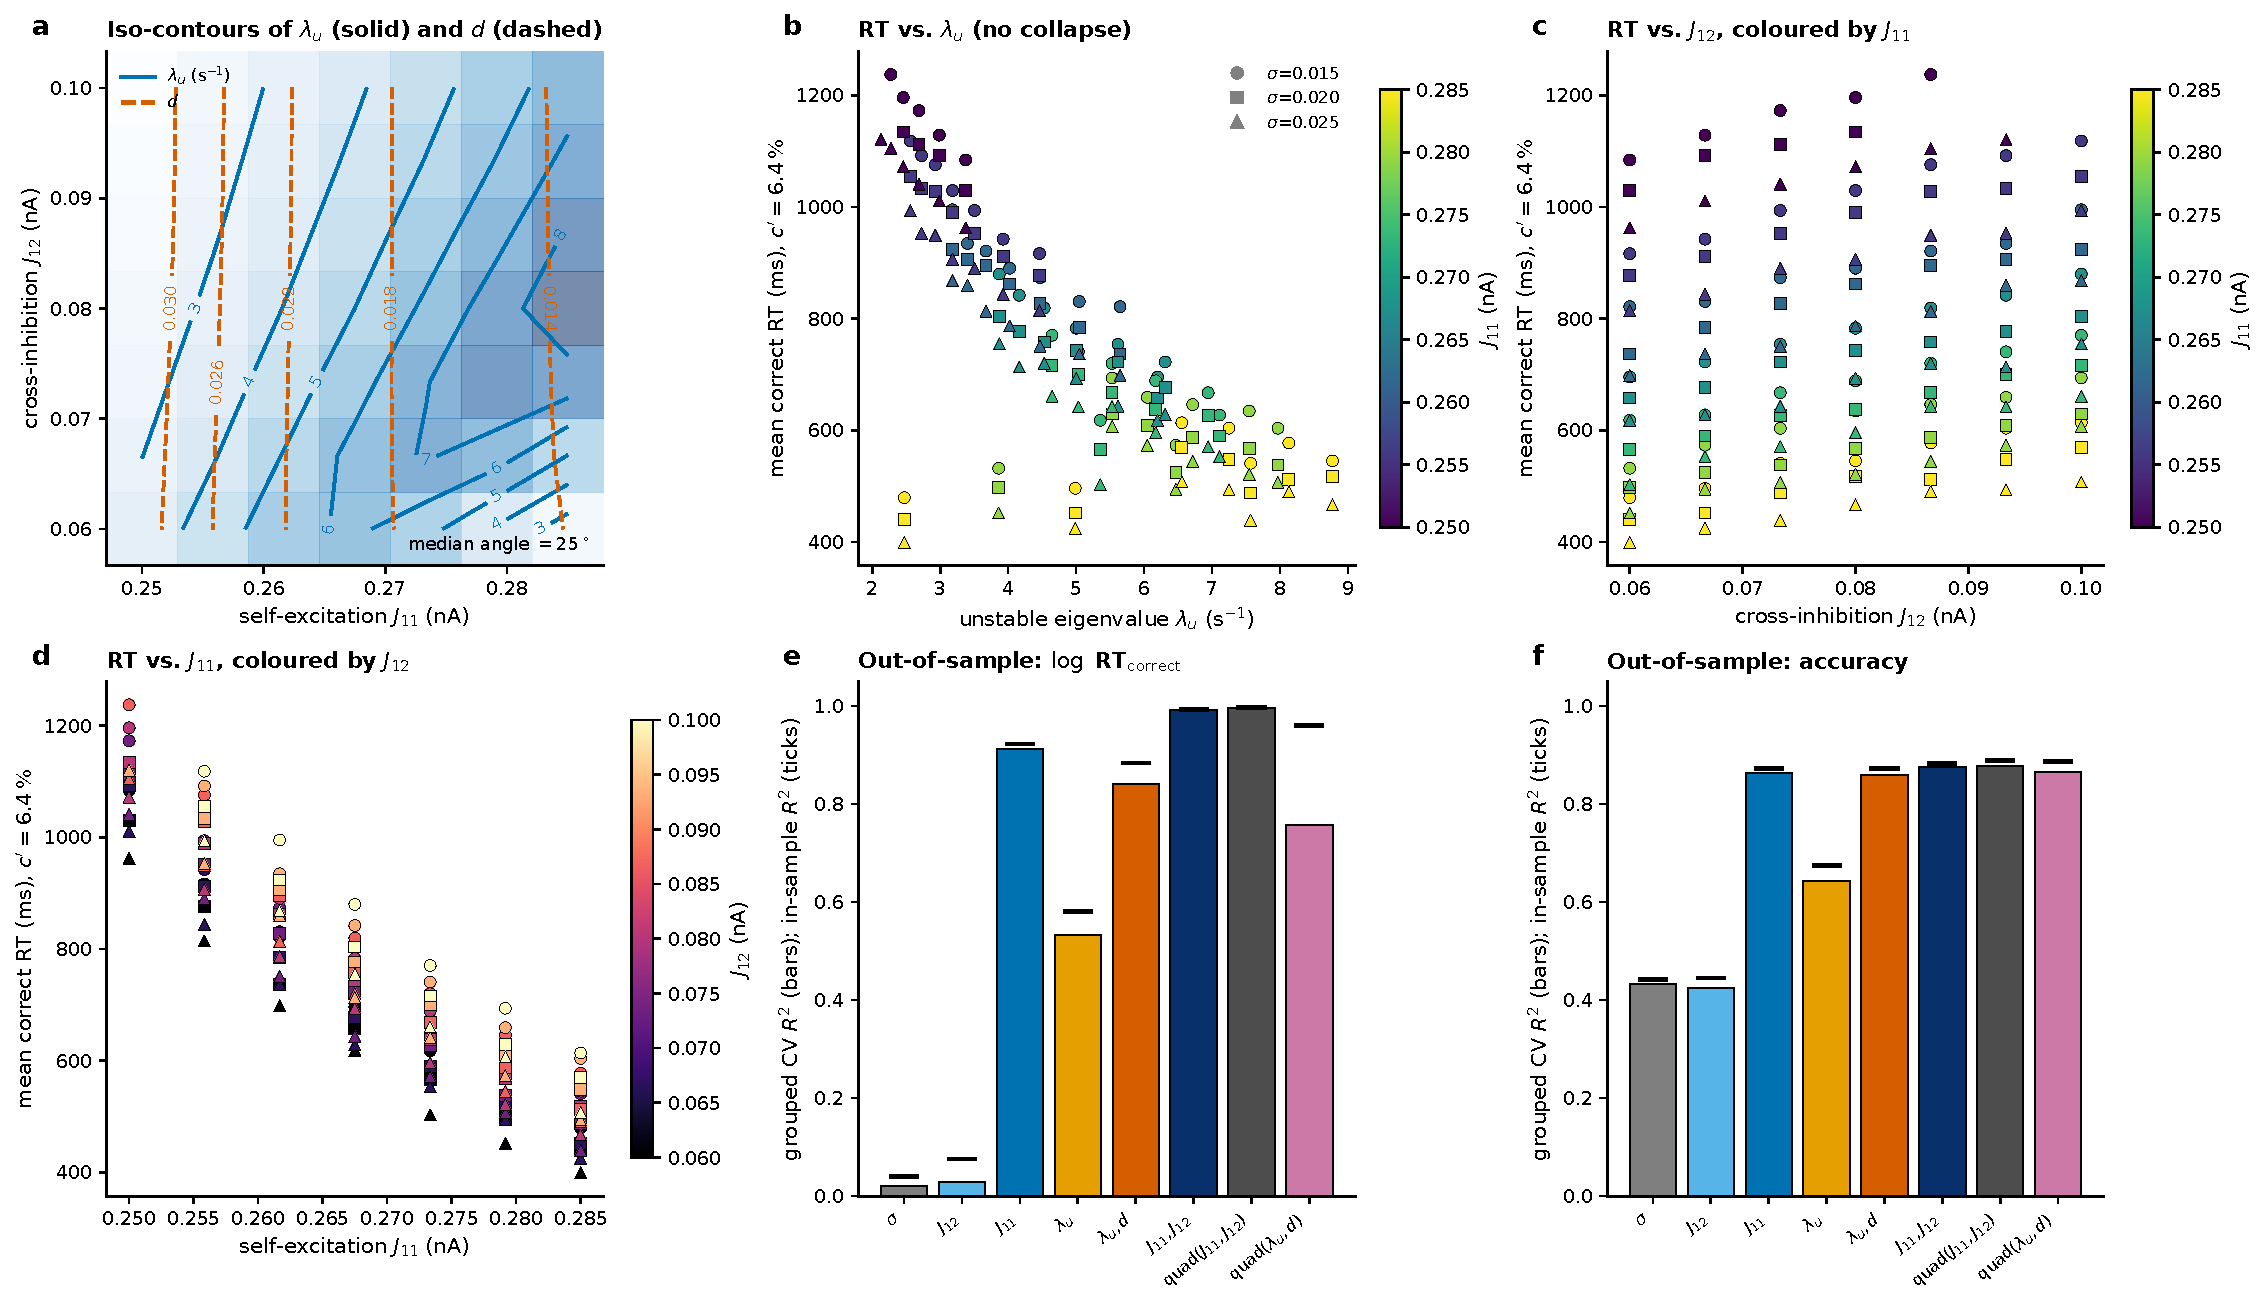
\includegraphics[width=\textwidth]{fig9_grid2d.pdf}
		\caption{Joint $(J_{11},J_{12})$ grid within the bistable winner-take-all region ($c'=\dCoh$\%). (a)~Transverse iso-contours of $\lambda_u$ (solid) and $d$ (dashed). (b--d)~Mean correct RT plotted against $\lambda_u$, $J_{12}$, and $J_{11}$ across three noise levels (marker shapes). (e,f)~Grouped cross-validated $R^2$ (bars) and in-sample $R^2$ (ticks) for $\log$ RT$_{\rm correct}$ and choice accuracy.}
		\label{fig:grid2d}
	\end{figure}
	On the $\dNGrid\times\dNGrid$ joint $(J_{11},J_{12})$ grid, all \dNCells{} of \dNTotal{} cells satisfy the bistable WTA criteria, providing $n=\dNRows$ circuit-by-noise observations. Across this grid, $\lambda_u$ ranges from \dLamLo{} to \dLamHi{} s$^{-1}$ and $d$ from \dDLo{} to \dDHi{}. Their iso-contours are transverse in the $(J_{11},J_{12})$ plane (median intersection angle \dAngle$^\circ$; \dFracAngle\% of cells above $30^\circ$; Fig.~\ref{fig:grid2d}a), yielding \dNEqPairs{} pairs of distinct circuits with nearly identical $\lambda_u$ (within 2\%) whose separatrix distances $d$ differ by up to \dMaxDD{}. Notably, the iso-contours of $d$ are nearly vertical: $d$ is almost purely a function of recurrent self-excitation $J_{11}$ (correlation $r=\dCorrDJeleven$ with $J_{11}$ versus $r=\dCorrDJtwelve$ with $J_{12}$), whereas $\lambda_u$ varies non-monotonically with both $J_{11}$ and $J_{12}$.
	
	\emph{Manifold collapse test.} If the local unstable eigenvalue $\lambda_u$ acted as a sufficient scalar invariant governing decision speed across circuit configurations, $\text{RT}_{\rm correct}$ at fixed noise would collapse onto a single curve when plotted against $\lambda_u$. It does not (Fig.~\ref{fig:grid2d}b): at fixed $\lambda_u$, RT is strongly stratified by $J_{11}$. Leave-one-circuit-out quadratic fits at each noise level (Table~\ref{tab:collapse}) show weak collapse for $\lambda_u$ alone (mean $R^2=\dCollapseLam$) and no collapse for $J_{12}$ alone (\dCollapseTw), but strong collapse onto $J_{11}$ alone (\dCollapseEl; Fig.~\ref{fig:grid2d}c,d).
	
	\begin{table}[t]\centering\small
		\begin{tabular}{rcccc}\toprule
			$\sigma$ (nA) & $n$ cells & $\lambda_u$ & $J_{11}$ & $J_{12}$\\\midrule
			0.015 & 47 & 0.46 & 0.90 & -0.09 \\
0.02 & 46 & 0.42 & 0.91 & -0.11 \\
0.025 & 48 & 0.52 & 0.92 & -0.08 \\
\bottomrule

		\end{tabular}
		\caption{Leave-one-cell-out $R^2$ of single-variable quadratic fits of $\log$ RT$_{\rm correct}$ on the 2D grid.}
		\label{tab:collapse}
	\end{table}
	\begin{table}[t]\centering\footnotesize
		\begin{tabular}{lccccc}\toprule
			Predictors & $R^2$ & CV $R^2$ & RMSE & CV RMSE & $\Delta$AIC\\\midrule
			$\sigma$ & 0.040 & 0.020 & 0.267 & 0.270 & 787.9 \\
$J_{12},\sigma$ & 0.076 & 0.028 & 0.262 & 0.269 & 784.6 \\
$J_{11},\sigma$ & 0.922 & 0.913 & 0.076 & 0.080 & 435.5 \\
$\log\lambda_u,\sigma$ & 0.580 & 0.533 & 0.177 & 0.186 & 673.2 \\
$\log\lambda_u,d,\sigma$ & 0.883 & 0.840 & 0.093 & 0.109 & 494.6 \\
$J_{11},J_{12},\sigma$ & 0.993 & 0.992 & 0.023 & 0.024 & 98.1 \\
quad$(J_{11},J_{12}),\sigma$ & 0.997 & 0.996 & 0.016 & 0.016 & 0.0 \\
quad$(\log\lambda_u,\log d),\sigma$ & 0.960 & 0.757 & 0.054 & 0.134 & 349.5 \\
$\log\lambda_u,J_{11},J_{12},\sigma$ & 0.993 & 0.993 & 0.023 & 0.023 & 98.2 \\
$\log d,\sigma$\,$^\dagger$ & 0.915 & 0.903 & 0.079 & 0.085 & 448.1 \\
\bottomrule

		\end{tabular}
		\caption{Joint 2D grid, $\log$ RT$_{\rm correct}$ (OLS). Grouped CV holds out whole $(J_{11},J_{12})$ circuit configurations across noise levels; RMSE in $\log$ units. $^\dagger$Exploratory post-hoc model.}
		\label{tab:2drt}
	\end{table}
	\begin{table}[t]\centering\footnotesize
		\begin{tabular}{lccccc}\toprule
			Predictors & pseudo-$R^2$ & CV & RMSE & CV RMSE & $\Delta$AIC\\\midrule
			$\sigma$ & 0.442 & 0.432 & 0.065 & 0.066 & 993.1 \\
$J_{12},\sigma$ & 0.445 & 0.424 & 0.065 & 0.066 & 988.3 \\
$J_{11},\sigma$ & 0.873 & 0.863 & 0.030 & 0.032 & 26.3 \\
$\log\lambda_u,\sigma$ & 0.675 & 0.642 & 0.049 & 0.051 & 472.4 \\
$\log\lambda_u,d,\sigma$ & 0.872 & 0.858 & 0.031 & 0.033 & 30.6 \\
$J_{11},J_{12},\sigma$ & 0.883 & 0.876 & 0.029 & 0.030 & 5.3 \\
quad$(J_{11},J_{12}),\sigma$ & 0.888 & 0.877 & 0.029 & 0.030 & 0.0 \\
quad$(\log\lambda_u,\log d),\sigma$ & 0.886 & 0.866 & 0.029 & 0.032 & 5.1 \\
$\log\lambda_u,J_{11},J_{12},\sigma$ & 0.883 & 0.876 & 0.029 & 0.030 & 7.3 \\
$\log d,\sigma$\,$^\dagger$ & 0.877 & 0.867 & 0.030 & 0.031 & 16.5 \\
\bottomrule

		\end{tabular}
		\caption{Joint 2D grid, choice accuracy (binomial regression); RMSE in probability units. $^\dagger$Exploratory.}
		\label{tab:2dacc}
	\end{table}
	
	\emph{Out-of-sample prediction across circuit configurations.} Grouped cross-validation on the 2D grid (Table~\ref{tab:2drt}) confirms that $\{\lambda_u,\sigma\}$ generalizes poorly across circuits (grouped CV $R^2=\ddRTLamCV$, compared with \ddRTSigCV{} for $\sigma$ alone and \ddRTJTwCV{} for $\{J_{12},\sigma\}$). By contrast, $\{J_{11},\sigma\}$ achieves grouped CV $R^2=\ddRTJElCV$ (and its post-hoc geometric counterpart $\{d,\sigma\}$ reaches \ddRTDCV), while including both circuit parameters in $\{J_{11},J_{12},\sigma\}$ yields the best out-of-sample prediction (grouped CV $R^2=\ddRTJJCV$; Table~\ref{tab:2drt}). Combining both saddle quantities in the linear model $\{\lambda_u,d,\sigma\}$ yields CV $R^2=\ddRTGeoCV$ (and adding $\lambda_u$ to $\{J_{11},J_{12},\sigma\}$ yields \ddRTLamJCV). To test whether the gap between linear $\{\lambda_u,d,\sigma\}$ and $\{J_{11},J_{12},\sigma\}$ reflects a nonlinear coordinate mapping between $(J_{11},J_{12})$ and $(\lambda_u,d)$, we also evaluated a full quadratic surface in $(\log\lambda_u,\log d)$: allowing quadratic curvature raises in-sample $R^2$ to \ddRTGeoQuadR{} (approaching the quadratic circuit model), but reduces out-of-sample grouped CV $R^2$ to \ddRTGeoQuadCV{} (versus \ddRTQuadCV{} for quadratic circuit parameters) because curved iso-contours near the bifurcation boundary create high-leverage cells when held out across folds. A similar ordering holds for choice accuracy (Table~\ref{tab:2dacc}), where noise is the primary driver (pseudo-$R^2=\ddAccSigR$ for $\sigma$ alone) and grouped CV rises from \ddAccLamCV{} ($\{\lambda_u,\sigma\}$) and \ddAccGeoCV{} ($\{\lambda_u,d,\sigma\}$) to \ddAccJElCV{} ($\{J_{11},\sigma\}$) and \ddAccJJCV{} ($\{J_{11},J_{12},\sigma\}$).
	
	\textbf{Mechanistic and statistical interpretation of H1.} Taken together, the 2D grid results demonstrate two key points. First, local saddle instability $\lambda_u$ alone cannot collapse decision speed across circuit configurations; instead, RT variation across the WTA regime is dominated by recurrent self-excitation $J_{11}$ (tracked geometrically by the separatrix distance $d$), with a secondary modulation by $J_{12}$. Second, the superior out-of-sample performance of linear $\{J_{11},J_{12},\sigma\}$ over $\{\lambda_u,d,\sigma\}$ reflects both a mathematical coordinate effect and a dynamical mechanism: (i)~mathematically, $\lambda_u(J_{11},J_{12})$ is a curved, non-monotone surface near the boundary of the WTA regime (Fig.~\ref{fig:grid2d}a), so linear regression in $(\log\lambda_u, d)$ underfits globally while quadratic regression in $(\log\lambda_u,\log d)$ captures the in-sample variance ($R^2=\ddRTGeoQuadR$) at the cost of boundary leverage in cross-validation; and (ii)~mechanistically, $(\lambda_u,d)$ measure only local geometry at the resting-to-saddle separatrix bottleneck, whereas $(J_{11},J_{12})$ also govern the post-saddle vector-field speed and choice-attractor depth that drive late-stage ramping across the downstream read-out threshold $\theta$ \citep{WongHuk2008, Standage2011}.
	
	\subsection{Testing H2: A tripartite dissociation between bifurcations, read-out, and behavior}
	\begin{figure}[t]\centering
		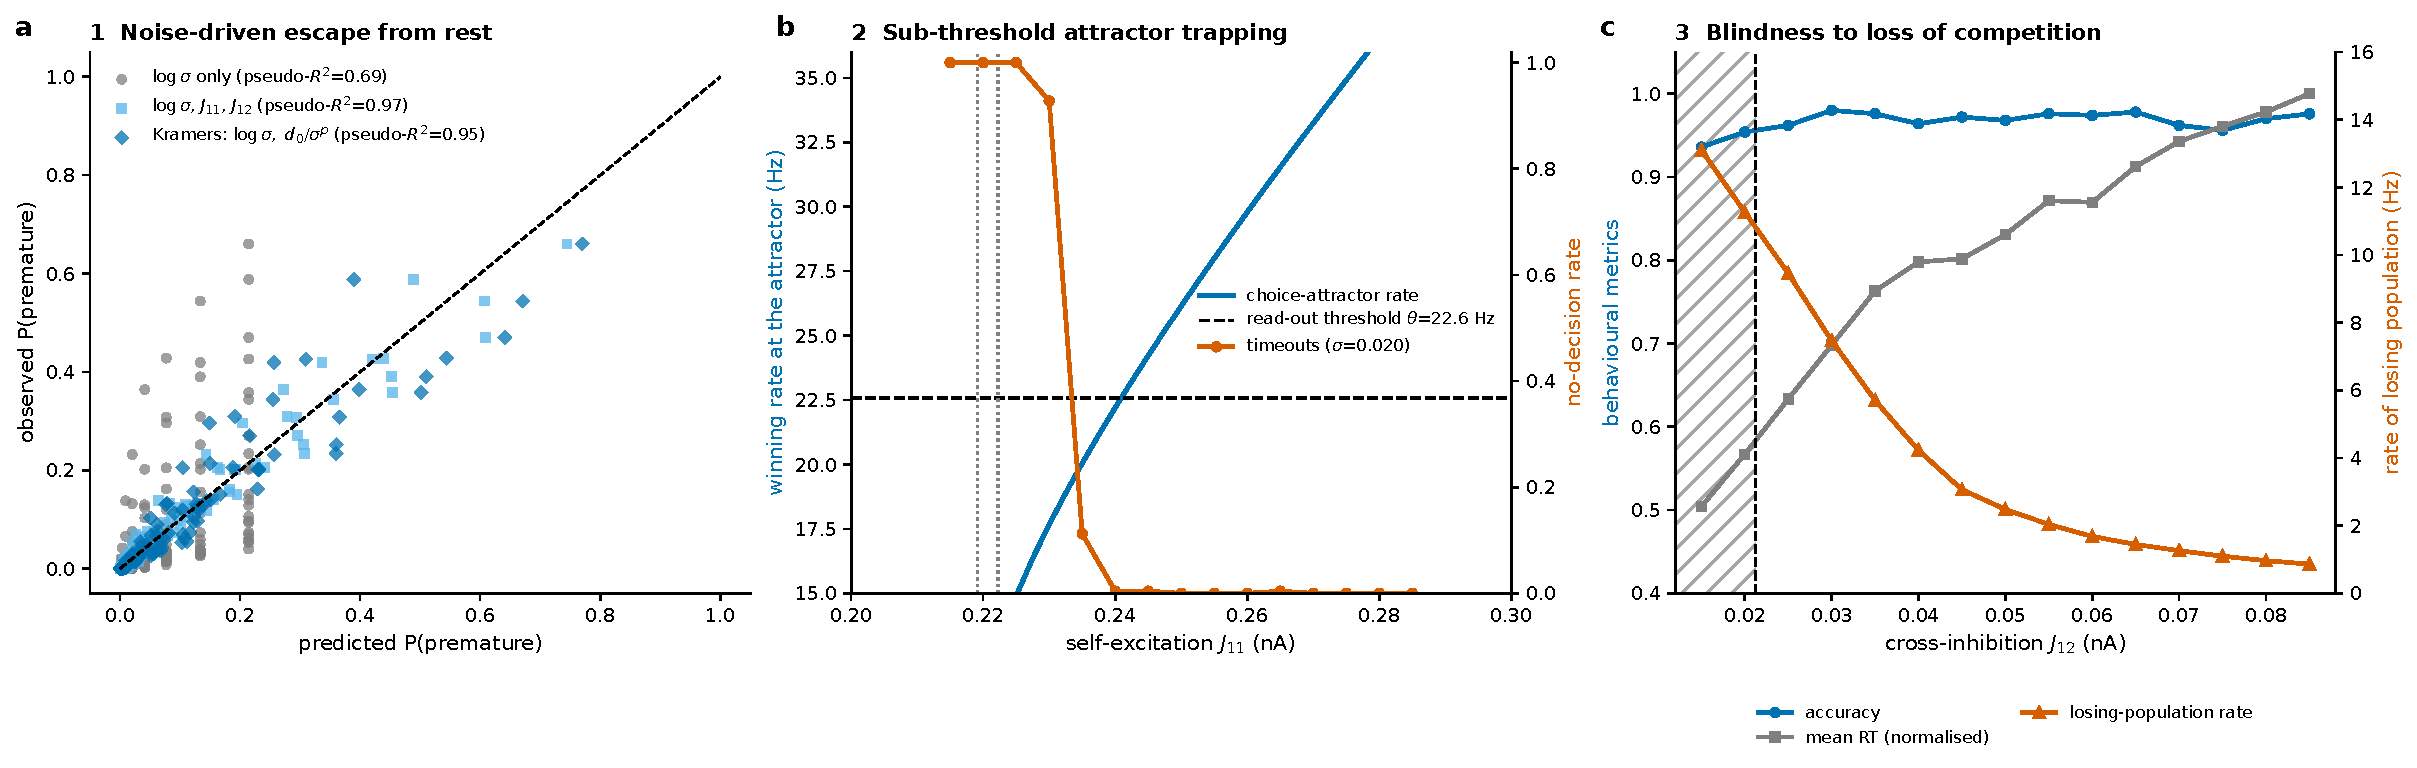
\includegraphics[width=\textwidth]{fig10_tripartite.pdf}
		\caption{Three dissociations between deterministic bifurcations and behavior. (a)~Observed versus predicted premature-response probability pooled across the $J_{12}$ and $J_{11}$ sweeps, illustrating Kramers-like scaling with the geometric barrier proxy $d_0$. (b)~Winning-attractor firing rate versus $J_{11}$ alongside the fixed read-out threshold $\theta$ (dashed) and empirical timeout rate at $\sigma=0.02$~nA (vertical dotted lines: saddle-node bifurcations). (c)~Along $J_{12}$ ($\sigma\approx0.02$ nA, 12.8\% coherence), accuracy and normalized RT vary smoothly into the hatched co-activation regime ($J_{12}<\bifJHiA$ nA), whereas the losing-population rate reveals the loss of competition.}
		\label{fig:tri}
	\end{figure}
	
	\subsubsection{Mechanism 1: Impulsivity reflects Kramers-like noise escape rather than resting-state bifurcation}
	Premature responses before stimulus onset could in principle result either from a bifurcation that destabilizes the resting state or from noise-activated escape across a stability barrier. Eigenvalue analysis shows that the pre-stimulus resting state remains locally stable in all \nRestTotal{} circuit configurations examined across all sweeps (\nPrestimUnstable{} unstable configurations; maximum eigenvalue \restLamMax{} s$^{-1}<0$). Thus, the impulsive regime is not triggered by a bifurcation of the resting state, but by noise-activated escape that becomes appreciable for $\sigma\gtrsim0.06$ nA (Fig.~\ref{fig:regime}c). Pooling the $J_{12}$ and $J_{11}$ sweeps (\premNCirc{} circuit configurations possessing a stimulus-free saddle, \premNRows{} total cells, \premNEvents{} with premature events), $\log\sigma$ alone gives pseudo-$R^2=\premSigR$, whereas the empirical Kramers-like model incorporating $d_0/\sigma^{p}$ reaches pseudo-$R^2=\premKPR$ and grouped-CV $R^2=\premKPCV$ (Table~\ref{tab:prem}, Fig.~\ref{fig:tri}a). The profiled exponent is $p=\premExp$, whereas fixing the classical gradient Kramers form $d_0^2/\sigma^2$ yields pseudo-$R^2=\premKTwoR$; this departure from simple quadratic scaling is expected because $d_0$ is a linear Euclidean distance in state space rather than a true potential energy barrier $\Delta U$, and because the two-population circuit is a non-gradient system driven by colored AMPA-filtered noise, justifying the designation of $d_0/\sigma^p$ as an empirical Kramers-like barrier scaling. Because the Euclidean barrier proxy $d_0$ (ranging from \premDLo{} to \premDHi{}) correlates with both $J_{11}$ ($r=\premCorrJeleven$) and $J_{12}$ ($r=\premCorrJtwelve$), it summarizes two-parameter circuit variation into a single geometric proxy at modest cost relative to the two-parameter circuit model $\{\log\sigma,J_{11},J_{12}\}$ (pseudo-$R^2=\premParR$, CV \premParCV; compared with \premDR{} for $d_0$ alone). Consistently, the noise level $\sigma$ at which 10\% or 20\% of trials terminate prematurely scales linearly with $d_0$ ($R^2=\premBTenR$ across $n=\premBTenN$ $J_{12}$ values for 10\%, Fig.~\ref{fig:regime}f; $R^2=\premBTwentyR$, $n=\premBTwentyN$ for 20\%).
	
	\begin{table}[t]\centering\small
		\begin{tabular}{lcccc}\toprule
			Predictors & pseudo-$R^2$ & CV & CV RMSE & $\Delta$AIC\\\midrule
			$\log\sigma$ & 0.69 & 0.68 & 0.073 & 10280 \\
$\log\sigma,J_{11},J_{12}$ & 0.97 & 0.96 & 0.023 & 353 \\
$\log\sigma$, quad$(J_{11},J_{12})$ & 0.98 & 0.98 & 0.018 & 0 \\
$d_0$ & 0.21 & 0.21 & 0.091 & 26885 \\
$\log\sigma,d_0$ & 0.95 & 0.94 & 0.039 & 1209 \\
$d_0^2/\sigma^2$ & 0.82 & 0.79 & 0.070 & 5756 \\
$\log\sigma,\,d_0/\sigma^{p}$ & 0.95 & 0.94 & 0.038 & 1082 \\
\bottomrule

		\end{tabular}
		\caption{Premature-response models pooled over the $J_{12}$ and $J_{11}$ sweeps (grouped CV holding out whole circuit configurations).}
		\label{tab:prem}
	\end{table}
	
	\subsubsection{Mechanism 2: Downstream circuit-to-readout mismatch causes indecisiveness prior to saddle-node bifurcation}
	\begin{figure}[t]\centering
		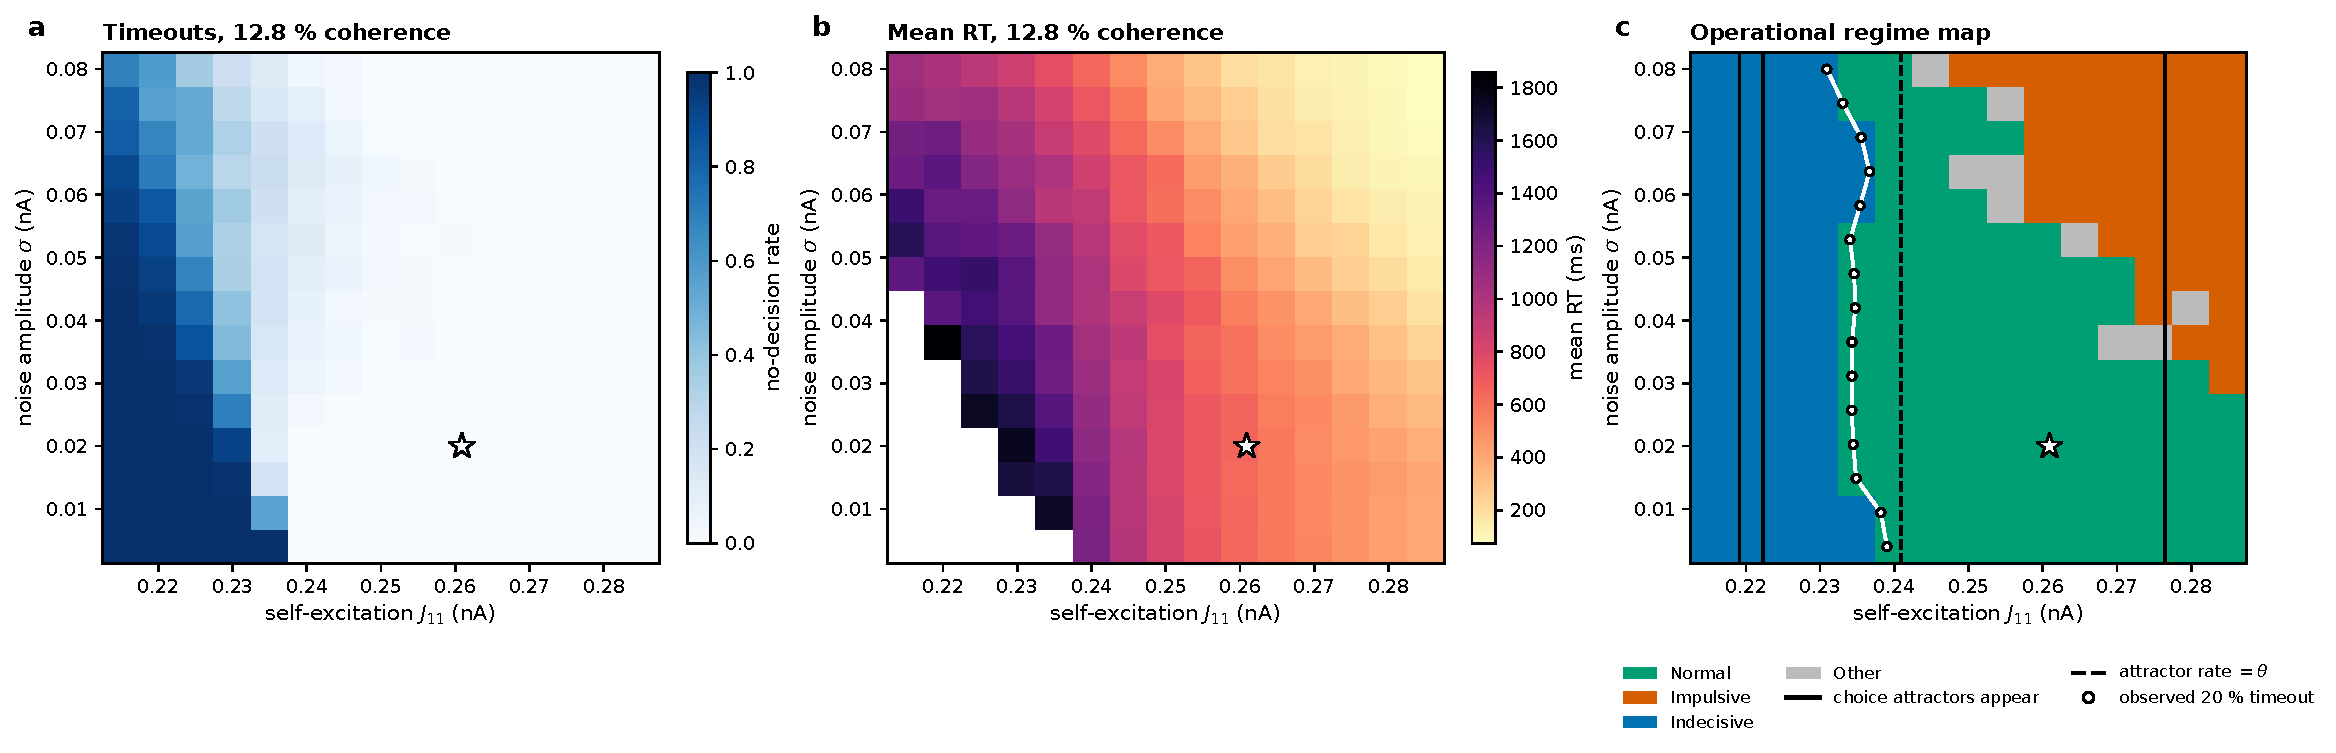
\includegraphics[width=\textwidth]{fig8_j11_sweep.pdf}
		\caption{$(J_{11},\sigma)$ sweep at 12.8\% coherence. (a) Timeout fraction. (b) Mean RT (white: no decisions). (c) Operational regime map showing the deterministic saddle-node bifurcations (solid lines), the coupling $J_{11}=\JelevenTheta$ nA where the winning-attractor rate equals the fixed read-out threshold $\theta$ (dashed line), and the observed 20\% timeout boundary.}
		\label{fig:j11}
	\end{figure}
	In computational psychiatry models of E/I dysfunction, behavioral indecisiveness (failure to commit within a trial) is often attributed to a loss of attractor stability or weakened evidence integration near a bifurcation \citep{Lam2022}. In our $(J_{11},\sigma)$ sweep, \regIndecEleven{} of \nCellsEleven{} cells are classified as indecisive (Fig.~\ref{fig:j11}), yet the observed 20\% timeout boundary lies at $J_{11}=\JelevenBoundLo$--\JelevenBoundHi{} nA---well \emph{above} the deterministic saddle-node bifurcations that destroy the choice attractors ($J_{11}=\bifElevenA$--$\bifElevenB$ nA) and just below the coupling $J_{11}=\JelevenTheta$ nA at which the steady-state winning-attractor firing rate falls below the downstream motor read-out threshold $\theta=\thetaHz$ Hz (Fig.~\ref{fig:tri}b, Fig.~\ref{fig:j11}c). Thus, indecisiveness in this regime does not reflect topological destruction of the choice attractors; rather, it arises from a \emph{circuit-to-readout mismatch} \citep{Standage2011, Standage2014} in which weakened recurrent excitation scales down the firing rate of the stable choice attractors below the level required to trigger an uncompensated downstream motor threshold. Trajectory analysis at $J_{11}=\trapJ$ nA (where the stable attractor rate is \trapRatt{} Hz $<\theta$) confirms this sub-threshold trapping: \trapPTO\% of trials ($n=\trapNTO$ of \trapN) time out, and at the end of these 2~s trials the leading population fires at \trapLead{} Hz on average, with \trapNear\% of timed-out trajectories residing within 3~Hz of the stable sub-threshold attractor rather than wandering near the saddle. Noise weakly shifts the timeout boundary toward lower $J_{11}$ by assisting threshold crossings (slope \JelevenShiftSlope{} nA per nA of $\sigma$, $R^2=\JelevenShiftR$), while varying the downstream threshold fraction $f\in\{0.6,0.75,0.9\}$ systematically shifts the number of indecisive cells (\regIndecElevenSixty, \regIndecElevenSeventyFive, and \regIndecElevenNinety{} cells, respectively).
	
	\subsubsection{Mechanism 3: Insensitivity of standard behavioral metrics to the loss of winner-take-all competition}
	When cross-inhibition is reduced below $J_{12}=\bifJHiA$ nA at 12.8\% coherence (corresponding to the region below the symmetric saddle-node $J_{12}=\bifJZeroA$ nA at 0\% coherence), the off-diagonal choice attractors are absent and the stimulus-driven circuit possesses only a single co-activation attractor in which both populations fire at high rates (hatched region in Figs.~\ref{fig:regime}e and \ref{fig:tri}c). Under stationary stimulus presentation at 12.8\% coherence ($\sigma\approx\coactSigma$ nA), standard first-crossing behavioral metrics remain insensitive to this loss of WTA competition: choice accuracy is \coactAccLow{} at the lowest $J_{12}$ versus \coactAccHigh{} at the highest $J_{12}$ (because asymmetric input drives the favored population across $\theta$ first), and mean RT varies smoothly from \coactRtLow{} to \coactRtHigh{} ms with no discontinuity at $J_{12}=\bifJHiA$ nA (Fig.~\ref{fig:tri}c). Operational behavioral criteria therefore label these non-competitive circuits as ``normal.'' In contrast, the neural population state at threshold crossing clearly distinguishes the regimes: the losing population fires at \coactLoserLow{} Hz at the lowest $J_{12}$ compared with \coactLoserHigh{} Hz at the highest $J_{12}$ (Fig.~\ref{fig:regime}d, Fig.~\ref{fig:tri}c), providing a direct neural signature of co-activation.
	
	\subsection{Empirical stationary density landscape and threshold sensitivity}\label{sec:sens}
	\begin{figure}[t]\centering
		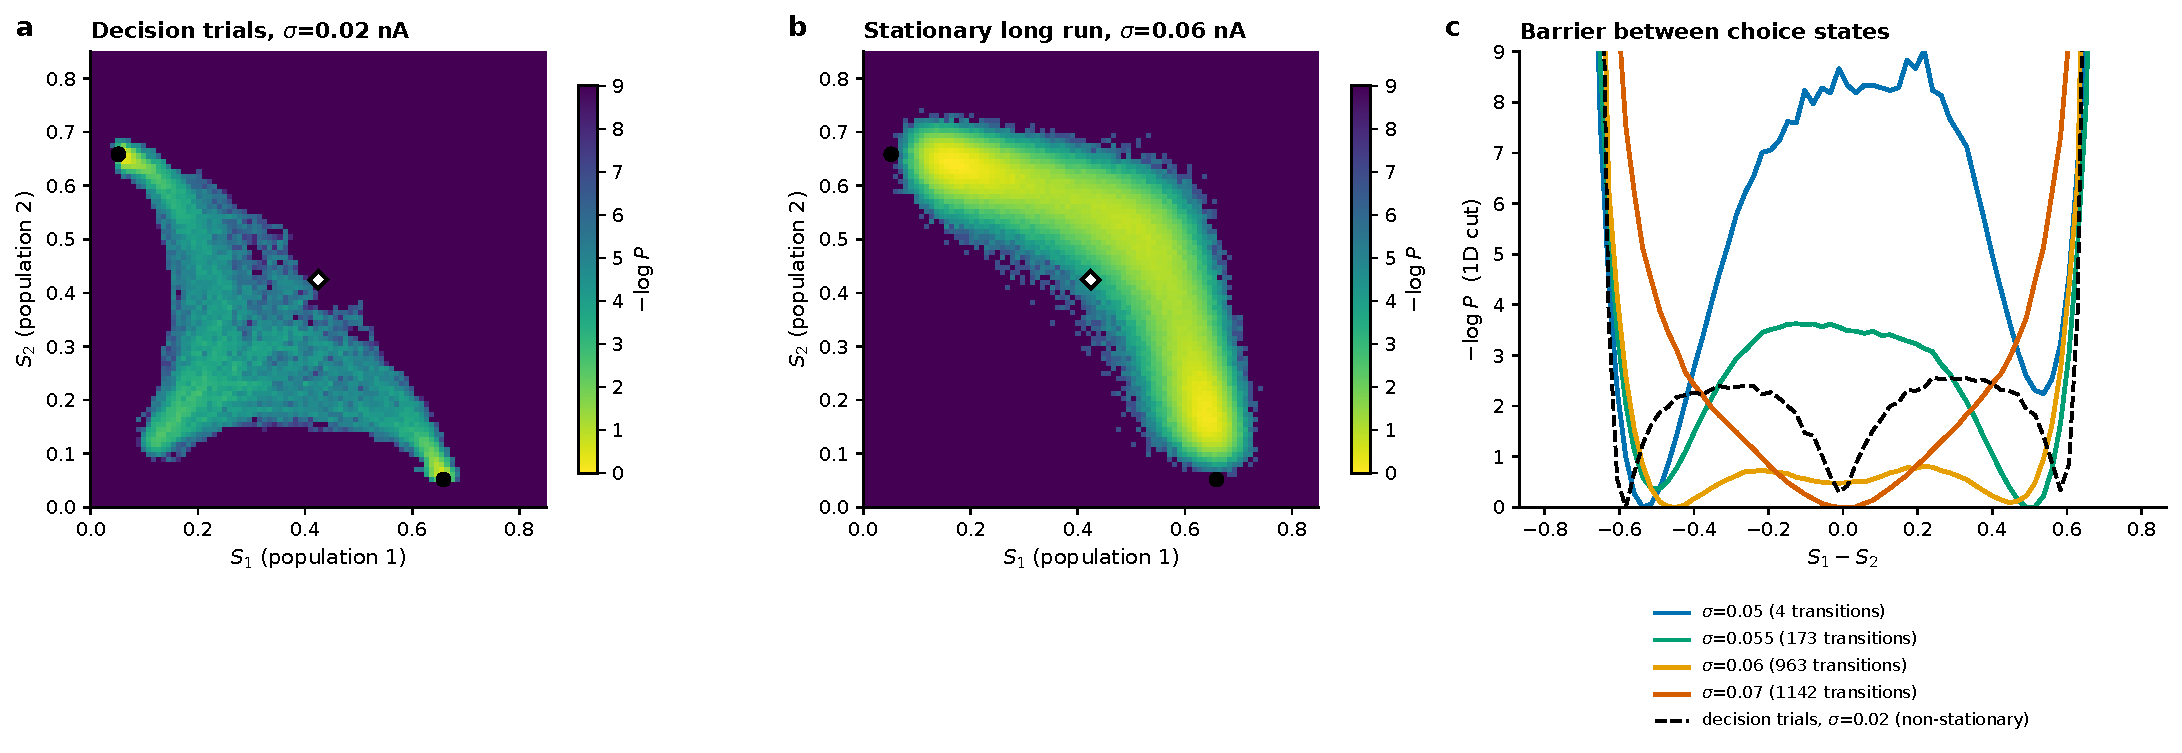
\includegraphics[width=\textwidth]{fig6_landscape.pdf}
		\caption{Empirical negative log density $-\log P(S_1,S_2)$ at 0\% coherence. (a) Non-stationary trajectory occupancy during decision trials at baseline noise. (b) Stationary density from a long run at $\sigma=0.06$ nA. (c) One-dimensional cuts along $S_1-S_2$ across noise levels.}
		\label{fig:land}
	\end{figure}
	\begin{figure}[t]\centering
		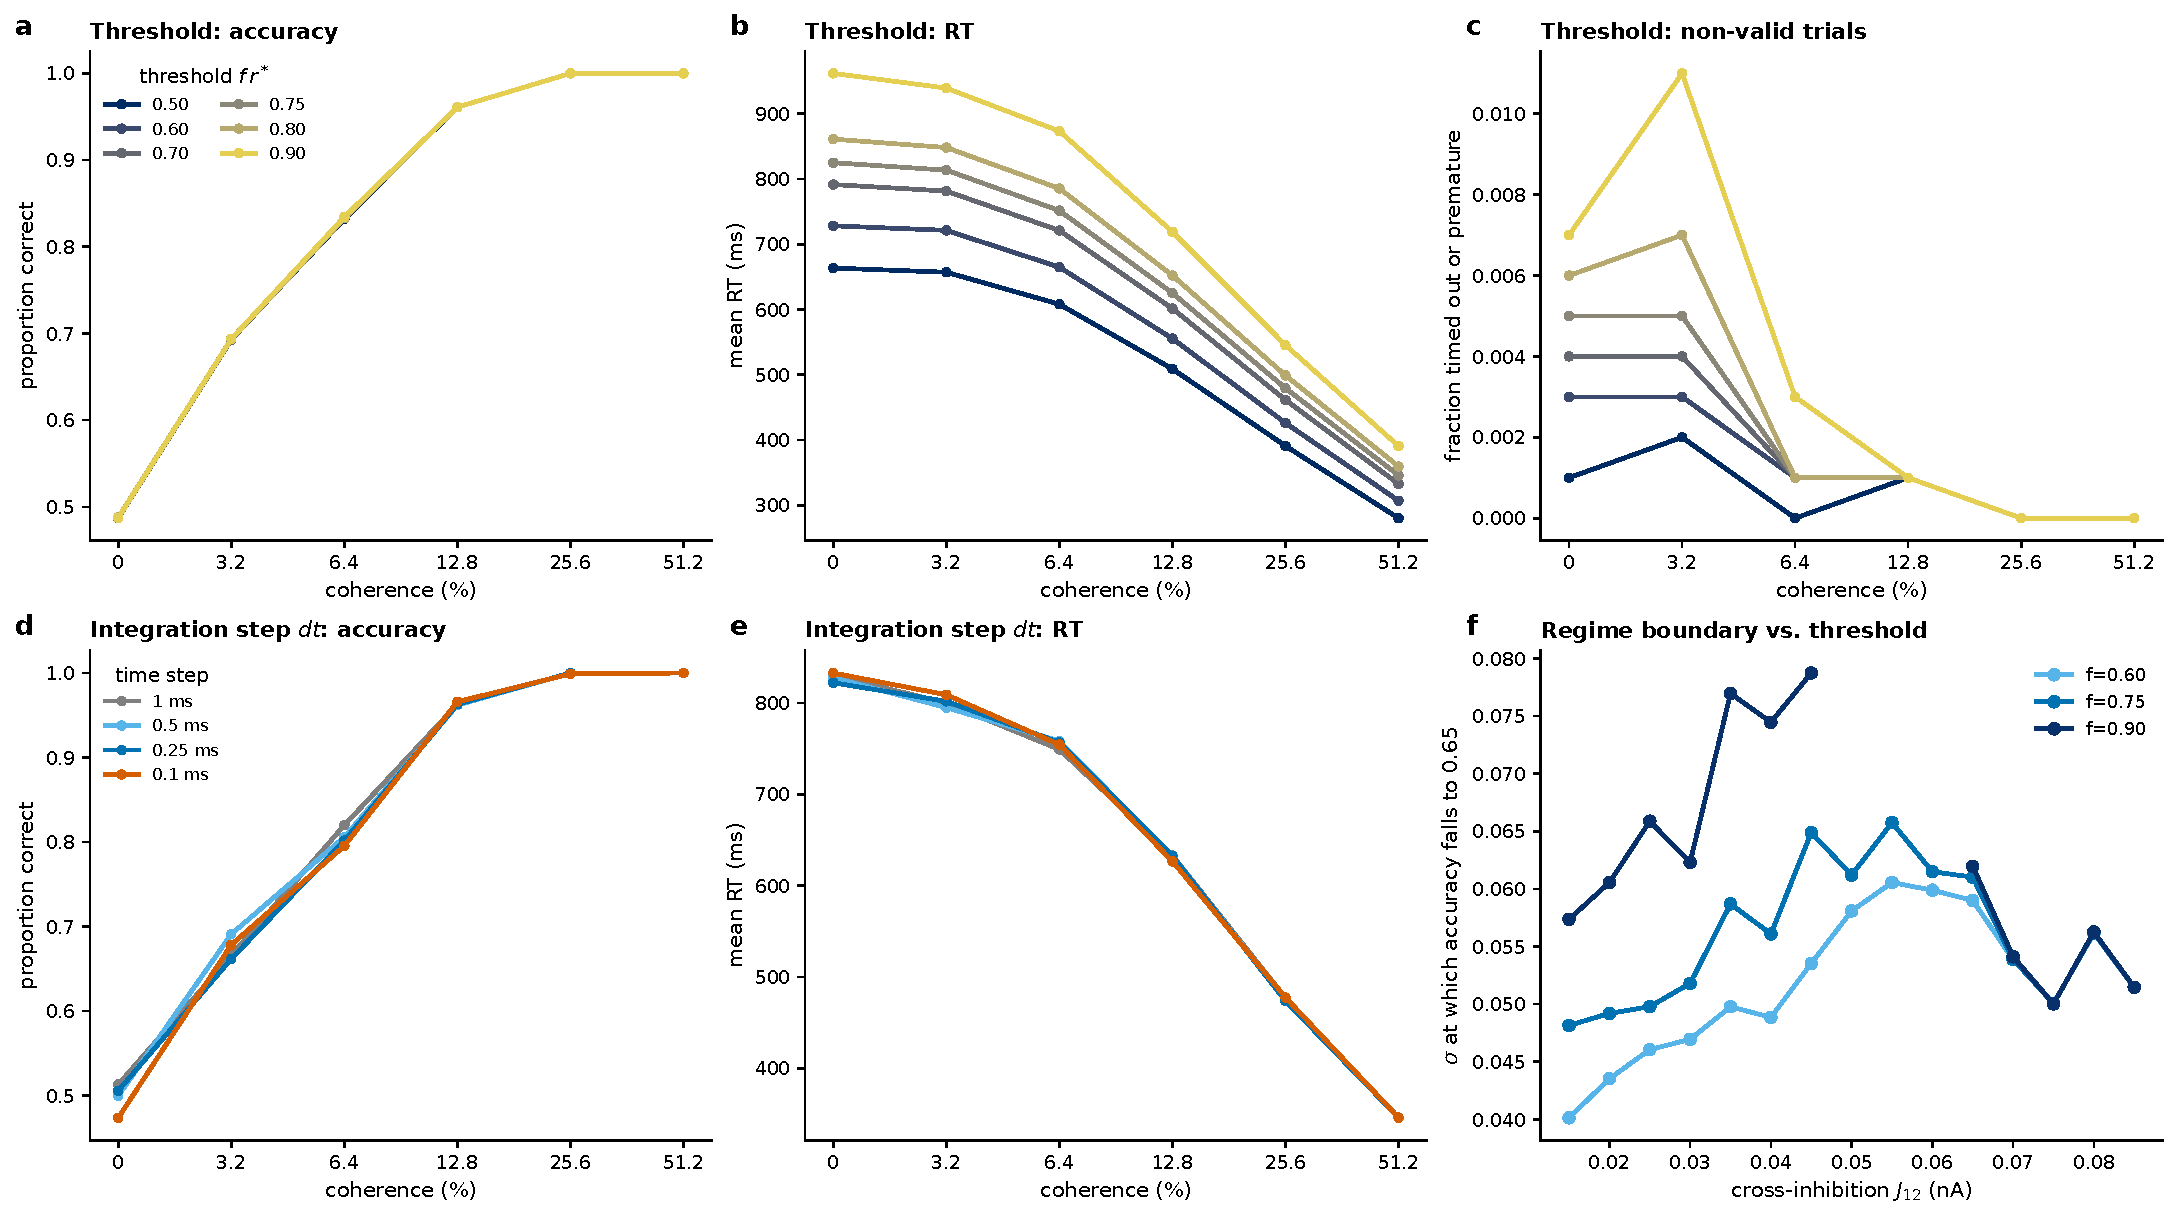
\includegraphics[width=\textwidth]{fig7_sensitivity.pdf}
		\caption{Sensitivity analyses. (a--c) Dependence of accuracy and RT on the read-out threshold fraction $f\in[0.5,0.9]$. (d,e) Numerical convergence across integration time steps $dt$. (f) Accuracy boundary in the $(J_{12},\sigma)$ plane across three threshold fractions.}
		\label{fig:sens}
	\end{figure}
	Because the two-population dynamics are non-gradient, $-\log P(S_1,S_2)$ estimated from long simulations ($\landT$~s each at 0\% coherence) represents an empirical negative log density landscape rather than an exact zero-noise Freidlin--Wentzell quasi-potential. These simulations show a bimodal double-well structure at moderate noise with rare noise-induced transitions between choice states (\nTransA{} transitions at $\sigma=0.05$ nA, \nTransB{} at $0.055$ nA, and \nTransC{} at $0.06$ nA), which merges into a single broad well at $\sigma=0.07$ nA (\nTransD{} transitions; Fig.~\ref{fig:land}). This empirical barrier collapse occurs in the same noise range ($\sigma\in[\sigAccLo,\sigAccHi]$ nA across $J_{12}$) where choice accuracy at 12.8\% coherence drops below 0.65; this breakdown noise level varies weakly and non-monotonically with $J_{12}$ (Spearman $\rho=\spAccRho$, $p=\spAccP$) without steps at the bifurcation lines. Finally, sensitivity checks confirm numerical convergence across integration steps $dt\in\{1,0.5,0.25,0.1\}$ ms (Fig.~\ref{fig:sens}d,e) and show that varying the read-out threshold fraction $f\in[0.5,0.9]$ leaves choice accuracy nearly unchanged (maximum spread \accSpreadF{}, since basin commitment occurs near the separatrix) while shifting mean RT at 0\% coherence from \rtZeroFLow{} ms ($f=\fLow$) to \rtZeroFHigh{} ms ($f=\fHigh$) and adjusting the count of impulsive cells (\regImpSixty, \regImpSeventyFive, and \regImpNinety{} of \nCells{} cells for $f=0.6,0.75,0.9$; Fig.~\ref{fig:sens}a--c,f).
	
	\section{Discussion}
	Our analysis separates two questions that are often conflated in reduced dynamical models of decision-making: how phase-plane geometry organizes stochastic behavior across circuit configurations, and whether behavioral regime boundaries coincide with structural bifurcations.
	
	\paragraph{Insufficiency of local saddle instability and the role of global attractor geometry in decision speed.}
	Analytical reductions of two-population attractor models to a one-dimensional nonlinear diffusion equation \citep{RoxinLedberg2008} focus on local dynamics near the pitchfork bifurcation, where the unstable eigenvalue $\lambda_u$ of the saddle sets the timescale of divergence. While a one-dimensional sweep along $J_{12}$ appears consistent with single-scalar control by $\lambda_u$ ($R^2=\HoneRTLamSigR$), our two-dimensional $(J_{11},J_{12})$ grid analysis shows that this agreement is an artifact of single-parameter collinearity. When $J_{11}$ and $J_{12}$ are varied jointly across the bistable WTA regime, $\lambda_u$ alone fails to collapse RT (grouped CV $R^2=\ddRTLamCV$). Instead, RT variation across the grid is dominated by recurrent self-excitation $J_{11}$ (CV $R^2=\ddRTJElCV$), which closely tracks the Euclidean resting-to-separatrix distance $d$ ($r=\dCorrDJeleven$), with cross-inhibition $J_{12}$ providing a secondary modulation (raising grouped CV $R^2$ to \ddRTJJCV{} for $\{J_{11},J_{12},\sigma\}$).
	
	Crucially, our comparison between linear and quadratic regressions resolves why the raw circuit parameters $\{J_{11},J_{12},\sigma\}$ outperform the local saddle coordinates $\{\lambda_u,d,\sigma\}$ (CV $R^2=\ddRTGeoCV$) out of sample. First, the mapping from $(J_{11},J_{12})$ to $(\lambda_u,d)$ is strongly nonlinear and non-monotone near the boundary of the WTA regime (Fig.~\ref{fig:grid2d}a); accounting for this curvature with a quadratic surface in $(\log\lambda_u,\log d)$ restores in-sample accuracy to $R^2=\ddRTGeoQuadR$, although boundary leverage degrades cross-validation across held-out circuits (CV $R^2=\ddRTGeoQuadCV$). Second, at a mechanistic level, $d$ and $\lambda_u$ measure only the initial escape across the separatrix bottleneck, whereas total reaction time also encompasses late-stage acceleration and ramping toward the choice attractor until crossing the downstream bound $\theta$---a phase directly governed by attractor depth and vector-field velocity set by $J_{11}$ and $J_{12}$ \citep{WongWang2006, WongHuk2008, Standage2011, Niyogi2013}. We do not claim that no geometric quantity can capture decision speed; rather, the two local saddle coordinates examined here ($\lambda_u$ and $d$) are insufficient across the two-dimensional circuit space without accounting for post-saddle attractor geometry. Consequently, E/I perturbations that simultaneously alter excitatory and inhibitory couplings \citep{Murray2014, Lam2022} cannot be reduced to a single scalar ratio $J_{11}/J_{12}$ or a single local saddle eigenvalue.
	
	\paragraph{Tripartite dissociation between structural bifurcations and behavioral phenotypes.}
	Across all three examined failure modes, behavioral transitions dissociate from deterministic bifurcations:
	\begin{enumerate}[leftmargin=*]
		\item \emph{Kramers-like pre-stimulus escape:} Impulsive premature responses emerge while the pre-stimulus resting attractor remains locally stable across all \nRestTotal{} circuit configurations, following an empirical Kramers-like scaling with the geometric barrier proxy $d_0/\sigma^p$ (grouped CV $R^2=\premKPCV$).
		\item \emph{Downstream circuit-to-readout mismatch:} Whereas computational psychiatry studies often attribute indecisive responding directly to weakened attractor stability or bifurcation crossing within the decision circuit \citep{Lam2022}, our results demonstrate that when downstream motor initiation requires crossing a stereotyped firing-rate threshold $\theta$ \citep{RoitmanShadlen2002, Kiani2008, Standage2014}, reducing $J_{11}$ produces timeouts well before saddle-node annihilation of the choice attractors. Thus, a mismatch between upstream attractor scaling and downstream read-out bounds is sufficient to generate an indecisive phenotype without any topological change in the phase portrait.
		\item \emph{Insensitivity of stationary first-crossing metrics to co-activation:} When $J_{12}$ drops below the bifurcation boundary ($J_{12}<\bifJHiA$ nA at 12.8\% coherence), WTA competition is lost in favor of high-rate co-activation, yet choice accuracy and first-crossing RT under stationary stimuli at 12.8\% coherence remain smooth and unimpaired. Detecting this loss of competition requires either monitoring neural population activity (specifically, the elevated firing rate of the losing population at commitment; Fig.~\ref{fig:tri}c, \citealp{Insabato2010}) or employing time-varying psychophysical perturbations such as brief motion pulses \citep{HukShadlen2005, Wong2007, WongHuk2008, Lam2022}.
	\end{enumerate}
	
	\paragraph{Methodological scope and limitations.}
	Analyzing the reduced two-variable model of \citet{WongWang2006} rather than a large-scale spiking network \citep{Wang2002, Lam2022} was a deliberate methodological choice that enabled high-accuracy numerical calculation of fixed points, Jacobian eigenvalues, and separatrices across dozens of circuit configurations. Several limitations and scope conditions should be noted. (i)~Operational regime classifications depend on preset cut-offs and on the fixed downstream read-out threshold $\theta$ (Section~\ref{sec:sens}); in particular, sub-threshold trapping at low $J_{11}$ diagnoses the consequences of an uncompensated downstream read-out bound, whereas biological circuits may partially compensate via homeostatic threshold adaptation or time-dependent urgency/gain modulation \citep{Standage2011, Niyogi2013, Hanks2014, Standage2014}. Moreover, our demonstration that accuracy and first-crossing RT are insensitive to the loss of WTA competition was evaluated under asymmetric stationary input (12.8\% coherence), where stimulus bias drives the favored population across $\theta$ first; how co-activation shapes RT distributions at 0\% coherence remains a complementary question. (ii)~Because the two-population vector field is non-gradient \citep{YeLi2021}, the Euclidean distances $d$ and $d_0$ and the empirical stationary density $-\log P$ are geometric and statistical proxies rather than exact minimum-action quasi-potentials. (iii)~In our statistical analyses, 5-fold grouped cross-validation holds out whole $(J_{11},J_{12})$ circuit configurations across noise levels to prevent data leakage, which tests interpolation across circuit configurations within the sampled grid rather than extrapolation to radically different dynamical regimes. (iv)~Finally, this study characterizes mechanistic principles in a canonical circuit model rather than fitting free parameters to individual empirical or clinical datasets.
	
	\section{Conclusion}
	In the reduced Wong--Wang decision circuit, deterministic phase-plane geometry organizes noise-driven behavior, whereas structural bifurcations fail to mark behavioral regime boundaries. We do not claim that no geometric quantity can capture decision speed; rather, the two local saddle coordinates examined here ($\lambda_u$ and $d$) are insufficient across two-dimensional $(J_{11},J_{12})$ perturbations, as RT is dominated by $J_{11}$ (controlling separatrix distance $d$ and post-saddle attractor depth relative to the read-out bound) with a secondary modulation by $J_{12}$. Furthermore, impulsive escape occurs without resting-state bifurcation, low-$J_{11}$ indecisiveness precedes saddle-node annihilation via a downstream circuit-to-readout mismatch, and under stationary stimuli at 12.8\% coherence, standard accuracy and first-crossing RT metrics are insensitive to the collapse of winner-take-all competition at weak cross-inhibition.
	
	\section*{Declarations}
	\paragraph{Funding.} The author received no specific grant or external financial support from any funding agency in the public, commercial, or not-for-profit sectors for this research.
	
	\paragraph{Competing Interests.} The author declares no competing financial or non-financial interests.
	
	\paragraph{Data and Code Availability.} All simulation data, analysis scripts, deterministic fixed-point and separatrix continuation routines, automated unit tests, and the generator for all LaTeX numerical macros (\texttt{generated\_numbers.tex}) are openly available at \url{https://github.com/alitkbbl/Decision-Circuit-Dynamics}. Running a single command (\texttt{python run\_all.py}) reproduces all tables, figures, and numerical values reported in this study from fixed random seeds.
	
	\paragraph{Use of AI-Assisted Technologies.} During the preparation of this work, large language models were used to assist with code development, debugging, and academic language editing. The author reviewed, verified, and validated all simulation and analysis code as well as the final manuscript text, and takes full responsibility for the scientific integrity and content of this publication.
	
	\appendix
\section{Model Parameters}\label{app:params}
\begin{center}\small
	\begin{tabular}{@{}llp{0.52\textwidth}@{}}\toprule
		Symbol & Value & Biophysical meaning\\\midrule
		$\tau_S$ & 100 ms & NMDA gating decay time constant\\
		$\gamma$ & 0.641 & NMDA saturation/kinetics factor\\
		$a,\,b,\,d_H$ & 270 Hz/nA, 108 Hz, 0.154 s & Input--output transfer function $H(x)$ parameters ($d_H$ denoted $d$ in \citealp{WongWang2006})\\
		$J_{11}$ & 0.2609 nA & Recurrent self-excitation coupling\\
		$J_{12}$ & 0.0497 nA & Effective cross-inhibition coupling\\
		$I_0$ & 0.3255 nA & Baseline background synaptic input\\
		$J_{\rm ext}$, $\mu_0$ & $5.2\times10^{-4}$ nA/Hz, 30 Hz & Stimulus coupling and reference firing rate\\
		$\sigma$, $\tau_{\rm AMPA}$ & 0.02 nA, 2 ms & Ornstein--Uhlenbeck noise amplitude and AMPA time constant\\\bottomrule
	\end{tabular}
\end{center}
	\begin{thebibliography}{99}
		\bibitem[Abbott and Chance(2005)]{AbbottChance2005}
		Abbott, L.~F. and Chance, F.~S. (2005).
		Drivers and modulators from push-pull and balanced synaptic input.
		\textit{Progress in Brain Research}, 149, 147--155.
		
		\bibitem[Bogacz et~al.(2006)]{Bogacz2006}
		Bogacz, R., Brown, E., Moehlis, J., Holmes, P., and Cohen, J.~D. (2006).
		The physics of optimal decision making: a formal analysis of models of performance in two-alternative forced-choice tasks.
		\textit{Psychological Review}, 113(4), 700--765.
		
		\bibitem[Brunel and Wang(2001)]{BrunelWang2001}
		Brunel, N. and Wang, X.-J. (2001).
		Effects of neuromodulation in a cortical network model of object working memory dominated by recurrent inhibition.
		\textit{Journal of Computational Neuroscience}, 11(1), 63--85.
		
		\bibitem[Deco et~al.(2013)]{Deco2013}
		Deco, G., Rolls, E.~T., Albantakis, L., and Romo, R. (2013).
		Brain mechanisms for perceptual and reward-related decision-making.
		\textit{Progress in Neurobiology}, 103, 194--213.
		
		\bibitem[Gillespie(1996)]{Gillespie1996}
		Gillespie, D.~T. (1996).
		Exact numerical simulation of the Ornstein-Uhlenbeck process and its integral.
		\textit{Physical Review E}, 54(2), 2084--2091.
		
		\bibitem[Gold and Shadlen(2007)]{GoldShadlen2007}
		Gold, J.~I. and Shadlen, M.~N. (2007).
		The neural basis of decision making.
		\textit{Annual Review of Neuroscience}, 30, 535--574.
		
		\bibitem[H{\"a}nggi et~al.(1990)]{Hanggi1990}
		H{\"a}nggi, P., Talkner, P., and Borkovec, M. (1990).
		Reaction-rate theory: fifty years after Kramers.
		\textit{Reviews of Modern Physics}, 62(2), 251--341.
		
		\bibitem[Hanks et~al.(2014)]{Hanks2014}
		Hanks, T., Kiani, R., and Shadlen, M.~N. (2014).
		A neural mechanism of speed-accuracy tradeoff in macaque area LIP.
		\textit{eLife}, 3, e02260.
		
		\bibitem[Huk and Shadlen(2005)]{HukShadlen2005}
		Huk, A.~C. and Shadlen, M.~N. (2005).
		Neural activity in macaque parietal cortex reflects temporal integration of visual motion signals during perceptual decision making.
		\textit{Journal of Neuroscience}, 25(45), 10420--10436.
		
		\bibitem[Insabato et~al.(2010)]{Insabato2010}
		Insabato, A., Pannunzi, M., Rolls, E.~T., and Deco, G. (2010).
		Confidence-related decision making.
		\textit{Journal of Neurophysiology}, 104(1), 539--547.
		
		\bibitem[Kiani et~al.(2008)]{Kiani2008}
		Kiani, R., Hanks, T.~D., and Shadlen, M.~N. (2008).
		Bounded integration in parietal cortex underlies decisions even when viewing duration is dictated by the environment.
		\textit{Journal of Neuroscience}, 28(12), 3017--3029.
		
		\bibitem[Kramers(1940)]{Kramers1940}
		Kramers, H.~A. (1940).
		Brownian motion in a field of force and the diffusion model of chemical reactions.
		\textit{Physica}, 7(4), 284--304.
		
		\bibitem[Lam et~al.(2022)]{Lam2022}
		Lam, N.~H., Borduqui, T., Hallak, J., Roque, A.~C., Anticevic, A., Krystal, J.~H., Wang, X.-J., and Murray, J.~D. (2022).
		Effects of altered excitation-inhibition balance on decision making in a cortical circuit model.
		\textit{Journal of Neuroscience}, 42(6), 1035--1053.
		
		\bibitem[Murray et~al.(2014)]{Murray2014}
		Murray, J.~D., Anticevic, A., Gancsos, M., Ichinose, M., Corlett, P.~R., Krystal, J.~H., and Wang, X.-J. (2014).
		Linking microcircuit dysfunction to cognitive impairment: effects of disinhibition associated with schizophrenia in a cortical working memory model.
		\textit{Cerebral Cortex}, 24(4), 859--872.
		
		\bibitem[Niyogi and Wong-Lin(2013)]{Niyogi2013}
		Niyogi, R.~K. and Wong-Lin, K. (2013).
		Dynamic excitatory and inhibitory gain modulation can produce flexible, robust and optimal decision-making.
		\textit{PLoS Computational Biology}, 9(6), e1003099.
		
		\bibitem[Palmer et~al.(2005)]{Palmer2005}
		Palmer, J., Huk, A.~C., and Shadlen, M.~N. (2005).
		The effect of stimulus strength on the speed and accuracy of a perceptual decision.
		\textit{Journal of Vision}, 5(5), 376--404.
		
		\bibitem[Ratcliff and McKoon(2008)]{RatcliffMcKoon2008}
		Ratcliff, R. and McKoon, G. (2008).
		The diffusion decision model: theory and data for two-choice decision tasks.
		\textit{Neural Computation}, 20(4), 873--922.
		
		\bibitem[Roitman and Shadlen(2002)]{RoitmanShadlen2002}
		Roitman, J.~D. and Shadlen, M.~N. (2002).
		Response of neurons in the lateral intraparietal area during a combined visual discrimination reaction time task.
		\textit{Journal of Neuroscience}, 22(21), 9475--9489.
		
		\bibitem[Roxin and Ledberg(2008)]{RoxinLedberg2008}
		Roxin, A. and Ledberg, A. (2008).
		Neurobiological models of two-choice decision making can be reduced to a one-dimensional nonlinear diffusion equation.
		\textit{PLoS Computational Biology}, 4(3), e1000046.
		
		\bibitem[Shadlen and Newsome(2001)]{ShadlenNewsome2001}
		Shadlen, M.~N. and Newsome, W.~T. (2001).
		Neural basis of a perceptual decision in the parietal cortex (area LIP) of the rhesus monkey.
		\textit{Journal of Neurophysiology}, 86(4), 1916--1936.
		
		\bibitem[Standage et~al.(2011)]{Standage2011}
		Standage, D., You, H., Wang, D.-H., and Dorris, M.~C. (2011).
		Gain modulation by an urgency signal controls the speed--accuracy trade-off in a network model of a cortical decision circuit.
		\textit{Frontiers in Computational Neuroscience}, 5, 7.
		
		\bibitem[Standage et~al.(2014)]{Standage2014}
		Standage, D., Blohm, G., and Dorris, M.~C. (2014).
		On the neural implementation of the speed-accuracy trade-off.
		\textit{Frontiers in Neuroscience}, 8, 236.
		
		\bibitem[Strogatz(2015)]{Strogatz2015}
		Strogatz, S.~H. (2015).
		\textit{Nonlinear Dynamics and Chaos: With Applications to Physics, Biology, Chemistry, and Engineering} (2nd ed.).
		Westview Press.
		
		\bibitem[Wang(1999)]{Wang1999}
		Wang, X.-J. (1999).
		Synaptic basis of cortical persistent activity: the importance of NMDA receptors to working memory.
		\textit{Journal of Neuroscience}, 19(21), 9587--9603.
		
		\bibitem[Wang(2002)]{Wang2002}
		Wang, X.-J. (2002).
		Probabilistic decision making by slow reverberation in cortical circuits.
		\textit{Neuron}, 36(5), 955--968.
		
		\bibitem[Wong and Huk(2008)]{WongHuk2008}
		Wong, K.-F. and Huk, A.~C. (2008).
		Temporal dynamics underlying perceptual decision making: insights from the interplay between an attractor model and parietal neurophysiology.
		\textit{Frontiers in Neuroscience}, 2(2), 245--254.
		
		\bibitem[Wong and Wang(2006)]{WongWang2006}
		Wong, K.-F. and Wang, X.-J. (2006).
		A recurrent network mechanism of time integration in perceptual decisions.
		\textit{Journal of Neuroscience}, 26(4), 1314--1328.
		
		\bibitem[Wong et~al.(2007)]{Wong2007}
		Wong, K.-F., Huk, A.~C., Shadlen, M.~N., and Wang, X.-J. (2007).
		Neural circuit dynamics underlying accumulation of time-varying evidence during perceptual decision-making.
		\textit{Frontiers in Computational Neuroscience}, 1, 6.
		
		\bibitem[Ye and Li(2021)]{YeLi2021}
		Ye, L. and Li, C. (2021).
		Quantifying the landscape of decision making from spiking neural networks.
		\textit{Frontiers in Computational Neuroscience}, 15, 740601.
	\end{thebibliography}
\end{document}